%%%%%%%% ICML 2026 SUBMISSION %%%%%%%%%%%%%%%%%%%%%%%%%%%%%%%%%%%%%%%%%%%%%%%%%%%%
% Converted from the report "SFPRM as an Operator-Split AKOrN: Exact
% Correspondences Between Spherical Fixed-Point Reasoning and Artificial
% Kuramoto Oscillatory Neurons" (sfprm_akorn_equivalence.pdf).
% Built on the ICML 2026 example template (icml2026.sty, version of 2025-10-29).
%%%%%%%%%%%%%%%%%%%%%%%%%%%%%%%%%%%%%%%%%%%%%%%%%%%%%%%%%%%%%%%%%%%%%%%%%%%%%%%%

\documentclass{article}

\usepackage{microtype}
\usepackage{graphicx}
\usepackage{subcaption}
\usepackage{booktabs}

\usepackage{hyperref}

% Attempt to make hyperref and algorithmic work together better:
\newcommand{\theHalgorithm}{\arabic{algorithm}}

% Blind version for review:
\usepackage{icml2026}
% Preprint: \usepackage[preprint]{icml2026}
% Camera-ready: \usepackage[accepted]{icml2026}

\usepackage{amsmath}
\usepackage{amssymb}
\usepackage{mathtools}
\usepackage{amsthm}
\usepackage[capitalize,noabbrev]{cleveref}

%%%%%%%%%%%%%%%%%%%%%%%%%%%%%%%%
% THEOREMS
%%%%%%%%%%%%%%%%%%%%%%%%%%%%%%%%
% Shared numbering through alias counters, so that cleveref names each environment correctly.
\usepackage{aliascnt}
\newcommand{\sharedtheorem}[2]{%
  \newaliascnt{#1}{theorem}\newtheorem{#1}[#1]{#2}\aliascntresetthe{#1}%
  \crefname{#1}{#2}{#2s}\Crefname{#1}{#2}{#2s}}
\theoremstyle{plain}
\newtheorem{theorem}{Theorem}[section]
\crefname{theorem}{Theorem}{Theorems}
\sharedtheorem{proposition}{Proposition}
\sharedtheorem{lemma}{Lemma}
\sharedtheorem{corollary}{Corollary}
\theoremstyle{definition}
\sharedtheorem{definition}{Definition}
\theoremstyle{remark}
\sharedtheorem{remark}{Remark}

%%%%%%%%%%%%%%%%%%%%%%%%%%%%%%%%
% MACROS
%%%%%%%%%%%%%%%%%%%%%%%%%%%%%%%%
\newcommand{\R}{\mathbb{R}}
\newcommand{\Sph}{\mathbb{S}}
\newcommand{\ip}[2]{\langle #1,\, #2\rangle}
\newcommand{\norm}[1]{\lVert #1\rVert}
\newcommand{\Proj}{\operatorname{P}}
\newcommand{\Norm}{\operatorname{Norm}}
\newcommand{\Ret}{\Pi}
\newcommand{\Slerp}{\operatorname{Slerp}}
\newcommand{\Exp}{\operatorname{Exp}}
\newcommand{\Log}{\operatorname{Log}}
\newcommand{\Attn}{\operatorname{Attn}}
\newcommand{\MLP}{\operatorname{MLP}}
\newcommand{\Id}{\mathrm{I}}
\newcommand{\diag}{\operatorname{diag}}
\newcommand{\tang}{\mathrm{T}}
\newcommand{\grad}{\operatorname{grad}}

\icmltitlerunning{SFPRM as an Operator-Split AKOrN}

\begin{document}

\twocolumn[
  \icmltitle{SFPRM as an Operator-Split AKOrN: Exact Correspondences Between\\
    Spherical Fixed-Point Reasoning and Kuramoto Oscillatory Neurons}

  % Author information is removed automatically in the blind version.
  \begin{icmlauthorlist}
    \icmlauthor{Anonymous Author}{anon}
  \end{icmlauthorlist}
  \icmlaffiliation{anon}{Anonymous Institution}
  \icmlcorrespondingauthor{Anonymous Author}{anon@example.com}

  \icmlkeywords{Fixed-point reasoning, looped transformers, Kuramoto oscillators, hypersphere, Riemannian optimization}

  \vskip 0.3in
]

\printAffiliationsAndNotice{}

\begin{abstract}
  Looped fixed-point reasoners and oscillator-based networks have developed separately, although both
  evolve unit vectors on spheres. We show that the Spherical Fixed-Point Reasoning Model (SFPRM) is,
  at the level of its update rule, a generalized network of Artificial Kuramoto Oscillatory Neurons
  (AKOrN) with zero natural frequency. Two elementary lemmas establish that normalized residual updates
  and spherical linear interpolation are exactly AKOrN Euler steps with state-dependent step sizes.
  Consequently, one SFPRM iteration is exactly an AKOrN step driven by the full recurrent map, its
  geodesic input injection and nGPT attention sub-layers are exactly AKOrN's stimulus and coupling
  steps, the iteration collapses to a single AKOrN step up to $O(\varepsilon^2)$ when step sizes are
  small, and the two forms share their linearization and hence SFPRM's damping window. We delineate
  where the models differ, read SFPRM's existence and convergence results as oscillator locking, and
  derive the locking condition of an oscillatory extension, showing also that a constant natural
  frequency can be absorbed into the recurrent block. The correspondence then suggests a model: an
  energy-based SFPRM whose recurrent map is a Riemannian gradient step on an explicit energy built
  from the geodesic injection, a symmetric attention energy with signed heads and hidden tokens, and
  a Hopfield memory. It inherits an energy that decreases at every iteration, convergence from any
  start with an a priori halting bound, a real Jacobian spectrum at halted states with the widest
  possible damping window, energy-based selection over random restarts, and training by conjugate
  gradient or equilibrium propagation. Reading the memory as a von Mises--Fisher mixture leads to a
  codebook variant whose readout is tied to answer prototypes and whose concentration is annealed
  over iterations. All identities are verified numerically. In a small Sudoku pilot the first energy
  model trains slowly and its energy does not rank solutions. The codebook variant matches SFPRM on
  $4\times4$ boards with one restart and lags it on $6\times6$, but its lowest-energy restart tracks
  the oracle on both, raising out-of-distribution accuracy from $74\%$ to $99\%$ on $4\times4$ and
  from $11\%$ to $88\%$ on $6\times6$ with $64$ restarts.
\end{abstract}

% ===========================================================================
\section{Introduction}
\label{sec:intro}

Looped, weight-tied models apply one block repeatedly and read their prediction from the state it
converges to, so that depth becomes an iteration count chosen per input
\citep{dehghani2019universal,bai2019deq}. Recent recurrent reasoners for puzzles such as Sudoku and
mazes follow this pattern \citep{wang2025hrm,jolicoeur2025trm}, and the Fixed-Point Reasoning Model
(FPRM) makes the loop an explicit damped fixed-point solve with residual-based halting
\citep{movahedi2026fprm}. Its spherical counterpart, SFPRM \citep{sfprm}, runs the same loop on the
unit hypersphere of the normalized Transformer nGPT \citep{loshchilov2025ngpt}: input injection and
damping become geodesic operations, boundedness holds by construction, input injection guarantees a
fixed point, and damping comes with an explicit step-size window.

A separate line of work builds networks from coupled oscillators. Artificial Kuramoto Oscillatory
Neurons (AKOrN) generalize the Kuramoto model \citep{kuramoto1984} to unit vectors in $N$ dimensions
that rotate at natural frequencies, interact through learned couplings and are driven by a
conditional stimulus \citep{miyato2025akorn}. Both families evolve unit vectors by moving along a
tangent direction and renormalizing, yet the connection between them has not been made precise. A
precise connection matters for two reasons: it lets results proved for one family (SFPRM's existence
and damping guarantees, AKOrN's energy and synchronization picture) be read in the language of the
other, and it identifies which oscillator mechanisms SFPRM already contains and which it lacks.

\paragraph{Contributions.}
\begin{itemize}
  \item Two lemmas showing that normalized residual updates and spherical linear interpolation are
        exactly AKOrN Euler steps with state-dependent step sizes (\cref{sec:lemmas}).
  \item An exact equivalence: one SFPRM iteration is an AKOrN step with $\Omega=0$, one oscillator per
        token and the full recurrent map as drive; geodesic injection and nGPT attention sub-layers are
        exactly AKOrN's stimulus and coupling steps, so an iteration is an operator-split AKOrN step
        (\cref{sec:correspondence}).
  \item A first-order collapse to a single AKOrN Euler step with explicit stimulus, coupling and
        self-drive, and an exact correspondence of linearizations that transfers SFPRM's damping window
        to the AKOrN form (\cref{sec:collapse,sec:linearization}).
  \item A delineation of the differences between the models, an oscillator reading of SFPRM's theory,
        and an oscillatory extension with its locking condition, together with the observation that a
        constant natural frequency can be absorbed into the recurrent block
        (\cref{sec:differences,sec:oscillatory}).
  \item An energy-based SFPRM whose recurrent map is a gradient step on an explicit energy, with
        a Lyapunov and halting guarantee from any start, a real Jacobian spectrum at halted states,
        energy-based voting over restarts, and conjugate-gradient or equilibrium-propagation
        training, and a codebook variant whose energy ranks solutions; a pilot study measures what
        the energy costs and what it buys (\cref{sec:energy}).
\end{itemize}
Our analysis concerns update rules. All identities are verified numerically (\cref{sec:numerics}),
and the energy-based model is tested in a small controlled experiment. \Cref{tab:summary}
summarizes the results.

\begin{table}[t]
  \caption{Summary of results. ``Exact'' statements hold for any step sizes satisfying stated
  positivity conditions.}
  \label{tab:summary}
  \vskip 0.1in
  \begin{center}
  \begin{small}
  \begin{tabular}{@{}p{0.6\columnwidth}ll@{}}
    \toprule
    Statement & Type & Where \\
    \midrule
    Renormalized residual step $=$ tangent step & exact & Lem.~\ref{lem:renorm} \\
    $\Slerp$ $=$ tangent step & exact & Lem.~\ref{lem:slerp} \\
    SFPRM iteration $=$ AKOrN step ($\Omega=0$, $N=d$) & exact & Thm.~\ref{thm:outer} \\
    Injection $=$ stimulus step & exact & Prop.~\ref{prop:injection} \\
    Attention sub-layer $=$ coupling step & exact & Prop.~\ref{prop:attention} \\
    Iteration $=$ composition of AKOrN steps & exact & Thm.~\ref{thm:splitting} \\
    Collapse to a single AKOrN step & $O(\varepsilon^2)$ & Thm.~\ref{thm:trotter} \\
    Shared linearization and damping window & exact & Cor.~\ref{cor:window} \\
    Constant $\Omega$ absorbed into the block & exact & Prop.~\ref{prop:absorb} \\
    Locking condition with natural frequencies & exact & Prop.~\ref{prop:adler} \\
    \midrule
    Energy SFPRM: gradient $=$ injection $+$ symmetric coupling $+$ memory & exact & Prop.~\ref{prop:energy-gradient} \\
    Energy descent, convergence, halting bound & exact & Thm.~\ref{thm:lyapunov} \\
    Real spectrum, window $\eta<2/\lambda_{\max}$ & exact & Prop.~\ref{prop:real-spectrum} \\
    Energy selection over restarts & exact & Prop.~\ref{prop:voting} \\
    \bottomrule
  \end{tabular}
  \end{small}
  \end{center}
  \vskip -0.1in
\end{table}

% ===========================================================================
\section{Related Work}
\label{sec:related}

\paragraph{Looped and fixed-point reasoners.} Universal Transformers share weights across depth
\citep{dehghani2019universal}, and deep equilibrium models compute the fixed point of a weight-tied
layer and differentiate through it implicitly \citep{bai2019deq}. Hierarchical and tiny recursive
models refine latent states with nested loops and deep supervision
\citep{wang2025hrm,jolicoeur2025trm}. FPRM replaces the hierarchy by a single damped fixed-point
loop with pre-norm, residual scaling and residual-based halting \citep{movahedi2026fprm}; SFPRM moves
this loop to the hypersphere \citep{sfprm}. Equilibrium Reasoners learn task-conditioned attractors
and scale test-time compute through depth and random restarts \citep{huang2026eqr}, and
\citet{daulbaev2026gfpr} constrain the state to products of simplices and analyse the Jacobian at
FPRM's halted states. We do not propose a new reasoner; we characterize SFPRM's update rule.

\paragraph{Normalized networks.} nGPT keeps every hidden vector on the unit sphere and folds each
sub-layer into the state by a normalized residual step with learned eigen learning rates
\citep{loshchilov2025ngpt}. SFPRM uses this block, and \cref{lem:renorm} is the observation that each
such step is a tangent step.

\paragraph{Oscillatory networks.} The Kuramoto model is the canonical model of synchronization
\citep{kuramoto1984,strogatz2000}, and its non-Abelian generalizations evolve unit vectors on
higher-dimensional spheres \citep{lohe2009}. Oscillatory recurrent networks exploit oscillator
dynamics for stable long-range memory \citep{rusch2021cornn} and for spatiotemporally structured
representations through travelling waves \citep{keller2023nwm}. AKOrN builds feed-forward and
recurrent networks from $N$-dimensional Kuramoto units \citep{miyato2025akorn}; Kuramoto phase
encodings modulate attention in vision transformers \citep{xiao2026kope}; and Continuous Thought
Machines use the synchronization of neural activity as their representation \citep{darlow2025ctm}.
Equilibrium propagation \citep{scellier2017ep} has been extended to learn natural frequencies of
Kuramoto networks at phase-locked equilibria \citep{ahmadi2026phase}.

% ===========================================================================
\section{Background}
\label{sec:background}

\Cref{app:prelim} gives a self-contained account of the mathematics used here: retractions and
Riemannian gradients, rotations, gradient flows, damped fixed-point iterations, nGPT and operator
splitting. We summarize the essentials.

\subsection{Geometry of the Sphere}
\label{sec:geometry}

Let $\Sph^{n-1}=\{z\in\R^n:\norm{z}=1\}$. Every $v\in\R^n$ splits at $z$ into a radial and a
tangential part,
\begin{equation}
  v = \ip{v}{z}\,z + \Proj_z v,\qquad \Proj_z v := (\Id-zz^\top)\,v,
  \label{eq:proj}
\end{equation}
where $\Proj_z$ projects onto the tangent space $\tang_z\Sph^{n-1}=\{v:\ip{v}{z}=0\}$. We write
$\Ret(y):=y/\norm{y}$ for normalization and $\theta=\angle(u,v):=\arccos\ip{u}{v}$. The exponential
and logarithm maps are
\begin{align}
  \Exp_u(w) &= \cos(\norm{w})\,u+\sin(\norm{w})\,\tfrac{w}{\norm{w}},\\
  \Log_u(v) &= \tfrac{\theta}{\sin\theta}\,\Proj_u v,
\end{align}
for $w\in\tang_u\Sph^{n-1}$ and $\theta\in(0,\pi)$,
and spherical linear interpolation is
\begin{equation}
  \Slerp_\eta(u,v) = \frac{\sin((1-\eta)\theta)}{\sin\theta}\,u + \frac{\sin(\eta\theta)}{\sin\theta}\,v,
  \quad \eta\in[0,1].
  \label{eq:slerp}
\end{equation}
For sequences $z=(z_1,\dots,z_T)$ all operators act token-wise; $\odot$ is the element-wise product.

\subsection{Kuramoto Oscillators and AKOrN}
\label{sec:akorn}

The Kuramoto model $\dot\theta_i=\omega_i+\sum_jK_{ij}\sin(\theta_j-\theta_i)$ becomes, for
$x_i=(\cos\theta_i,\sin\theta_i)$ and the $90^\circ$ rotation $R$,
\begin{equation}
  \dot x_i = \omega_i R\,x_i + \Proj_{x_i}\Big(\sum_j K_{ij}x_j\Big),
  \label{eq:kuramoto-vector}
\end{equation}
since $\Proj_{x_i}x_j=\sin(\theta_j-\theta_i)\,Rx_i$ (\cref{app:kuramoto}). AKOrN
\citep{miyato2025akorn} generalizes this to oscillators $x_i\in\Sph^{N-1}$, typically with $N\in\{2,4\}$:
\begin{equation}
  \dot x_i = \Omega_i x_i + \Proj_{x_i}\Big(c_i + \sum_j J_{ij} x_j\Big),
  \label{eq:akorn-ode}
\end{equation}
with antisymmetric natural frequencies $\Omega_i$, couplings $J_{ij}$ (a convolution or attention) and
a conditional stimulus $c_i$. We call $c_i+\sum_jJ_{ij}x_j$ the \emph{drive}. The discrete update with
learned step size $\gamma>0$ is
\begin{equation}
  x_i \leftarrow \Ret\Big(x_i + \gamma\Big[\Omega_i x_i + \Proj_{x_i}\Big(c_i + \sum_j J_{ij}x_j\Big)\Big]\Big).
  \label{eq:akorn-step}
\end{equation}
For $\Omega=0$ and symmetric couplings $J_{ij}=J_{ji}^\top$,
\begin{equation}
  E(x) = -\tfrac12\textstyle\sum_{i,j} x_i^\top J_{ij} x_j - \sum_i c_i^\top x_i
  \label{eq:akorn-energy}
\end{equation}
is a Lyapunov function of \eqref{eq:akorn-ode}. A network stacks $L$ blocks of $T$ steps, passing a
norm-based readout of each block as the next stimulus; it is trained by backpropagation through
time, and on Sudoku clue cells start at $x=c$, the remaining cells start randomly, and test-time
predictions are selected by energy-based voting over random initializations.

\subsection{SFPRM}
\label{sec:sfprm}

SFPRM \citep{sfprm} keeps the state on $\mathcal S:=(\Sph^{d-1})^T$; the input $x\in\mathcal S$ is
the token-wise normalized embedding. One iteration reads
\begin{align}
  \tilde z_i &= F_\theta(z_i;x) := f_\theta\big(\Slerp_\lambda(z_i,x)\big), \label{eq:sfprm-inject}\\
  z_{i+1} &= \Slerp_{\eta_i}(z_i,\tilde z_i), \label{eq:sfprm-damp}
\end{align}
(geodesic injection and geodesic damping), and the solver halts when
$\max_t 1-\ip{z_{i,t}}{\tilde z_{i,t}}<\tau_c$. The damping $\eta_i$ starts at $1$ and is decayed by a
patience rule. The weight-tied network $f_\theta$ is a stack of $D$ nGPT layers, each consisting of
\begin{align}
  h &\leftarrow \Norm\big(h + \alpha_A\odot(\Norm(\Attn(h)) - h)\big),\label{eq:ngpt-attn}\\
  h &\leftarrow \Norm\big(h + \alpha_M\odot(\Norm(\MLP(h)) - h)\big),\label{eq:ngpt-mlp}
\end{align}
with per-coordinate eigen learning rates $\alpha_A,\alpha_M\in\R^d$. Multi-head attention with
QK-normalization has the form of an AKOrN coupling with state-dependent weights,
\begin{equation}
  \begin{split}
  \Attn(h)_t &= \textstyle\sum_{s=1}^T J_{ts}(h)\,h_s,\\
  J_{ts}(h) &:= \textstyle\sum_{k=1}^{H} a^{k}_{ts}(h)\,W_O^{k} W_V^{k},
  \end{split}
  \label{eq:attn-as-coupling}
\end{equation}
where $a^k_{ts}(h)$ are the softmax weights of head $k$.

% ===========================================================================
\section{Every Spherical Update Is a Tangent Step}
\label{sec:lemmas}

\begin{lemma}[Renormalized residual updates]
\label{lem:renorm}
Let $z\in\Sph^{n-1}$ and $w\in\R^n$ with $1+\ip{w}{z}>0$. Then
\begin{equation}
  \Ret(z+w) = \Ret\Big(z + \frac{1}{1+\ip{w}{z}}\,\Proj_z w\Big).
\end{equation}
\end{lemma}
\begin{proof}
By \eqref{eq:proj}, $z+w=(1+\ip{w}{z})\,z+\Proj_z w$, and $\Ret(\beta y)=\Ret(y)$ for $\beta>0$.
\end{proof}

\begin{lemma}[Slerp is a tangent step]
\label{lem:slerp}
Let $u,v\in\Sph^{n-1}$, $\theta=\angle(u,v)\in(0,\pi)$ and $\eta\in[0,1]$. Then
$\Slerp_\eta(u,v)=\Exp_u(\eta\Log_u v)$, and if $\eta\theta<\pi/2$,
\begin{equation}
  \Slerp_\eta(u,v) = \Ret\big(u + \gamma_\eta(\theta)\,\Proj_u v\big),
  \quad
  \gamma_\eta(\theta) := \frac{\tan(\eta\theta)}{\sin\theta}.
  \label{eq:gamma-eta}
\end{equation}
As $\theta\to0$, $\gamma_\eta(\theta)\to\eta$; at $\eta=1$, $\gamma_1(\theta)=1/\cos\theta$.
\end{lemma}
\begin{proof}
Let $e:=\Proj_uv/\sin\theta$, a unit tangent vector, so $v=\cos\theta\,u+\sin\theta\,e$. In
\eqref{eq:slerp} the coefficient of $u$ is
$[\sin((1-\eta)\theta)+\sin(\eta\theta)\cos\theta]/\sin\theta=\cos(\eta\theta)$ and that of $e$ is
$\sin(\eta\theta)$, so $\Slerp_\eta(u,v)=\cos(\eta\theta)u+\sin(\eta\theta)e=\Exp_u(\eta\Log_uv)$. If
$\eta\theta<\pi/2$ then $\cos(\eta\theta)>0$, and dividing by it gives
$\Ret(u+\tan(\eta\theta)\,e)=\Ret(u+\gamma_\eta(\theta)\Proj_uv)$.
\end{proof}

\begin{remark}[Only the angle differs]
\label{rem:angle}
All these updates move the state along the great circle through $z$ in a tangent direction and differ
only in the angle: $\Ret(z+\gamma\Proj_zh)$ rotates by $\arctan(\gamma\norm{\Proj_zh})<\pi/2$,
$\Slerp_\eta(z,v)$ by $\eta\angle(z,v)$, and $\Ret(z+w)$ by
$\operatorname{atan2}(\norm{\Proj_zw},1+\ip{w}{z})$. The positivity conditions exclude exactly the
rotations by $\pi/2$ or more, which the AKOrN form cannot produce with $\gamma>0$.
\end{remark}

% ===========================================================================
\section{SFPRM Is an Operator-Split AKOrN}
\label{sec:correspondence}

\begin{definition}[Generalized AKOrN step]
\label{def:gen-akorn}
Given a step size $\gamma>0$ (possibly state-dependent), an antisymmetric $\Omega$ and a drive
$D:\mathcal S\to(\R^d)^T$, define token-wise on $\mathcal S$
\begin{equation}
  \mathcal A_{\gamma,\Omega,D}(z) := \Ret\big(z + \gamma\,[\,\Omega z + \Proj_z D(z)\,]\big).
\end{equation}
AKOrN's update \eqref{eq:akorn-step} is the case $D(x)=c+Jx$ with constant $\gamma$, applied to
oscillators of dimension $N$.
\end{definition}

\subsection{One Iteration Is Exactly One AKOrN Step}

\begin{theorem}[Exact outer equivalence]
\label{thm:outer}
Let $\theta_{i,t}:=\angle(z_{i,t},\tilde z_{i,t})$ and assume $\eta_i\theta_{i,t}<\pi/2$ for all $t$.
Then the SFPRM iteration \eqref{eq:sfprm-inject}--\eqref{eq:sfprm-damp} satisfies
\begin{equation}
  z_{i+1,t} = \Ret\big(z_{i,t} + \gamma_{i,t}\,\Proj_{z_{i,t}} F_\theta(z_i;x)_t\big),
\end{equation}
with $\gamma_{i,t}=\tan(\eta_i\theta_{i,t})/\sin\theta_{i,t}$ ($\gamma_{i,t}:=\eta_i$ if
$\theta_{i,t}=0$). That is, $z_{i+1}=\mathcal A_{\gamma_i,0,F_\theta(\cdot;x)}(z_i)$: an AKOrN step
with $\Omega=0$, one oscillator per token ($N=d$), drive $c+Jz:=F_\theta(z;x)$, and an
angle-dependent step size.
\end{theorem}
\begin{proof}
Apply \cref{lem:slerp} token-wise to \eqref{eq:sfprm-damp} with $u=z_{i,t}$, $v=\tilde z_{i,t}$.
\end{proof}

\begin{corollary}[Fixed points]
\label{cor:fixed}
For any positive step size, the fixed points of $\mathcal A_{\gamma,0,F_\theta}$ are the states with
$F_\theta(z;x)_t=\pm z_t$ for all $t$. The fixed points of SFPRM are those with $F_\theta(z;x)=z$; the
antipodal solutions are excluded because $\Slerp$ is undefined there. The step size (SFPRM's $\eta_i$
or AKOrN's $\gamma$) never changes the solution set.
\end{corollary}

\subsection{Inside the Iteration, Every Operation Is an AKOrN Step}

\begin{proposition}[Geodesic injection is the stimulus step]
\label{prop:injection}
Let $\theta^x_t:=\angle(z_t,x_t)$ and assume $\lambda\theta^x_t<\pi/2$ (automatic for $\lambda\le1/2$).
Then $\Slerp_\lambda(z,x)_t=\Ret\big(z_t+\gamma_\lambda(\theta^x_t)\,\Proj_{z_t}x_t\big)$: an AKOrN
step with stimulus $c=x$, no coupling, and $\Omega=0$.
\end{proposition}
\begin{proof}
\cref{lem:slerp} with $u=z_t$, $v=x_t$, $\eta=\lambda$.
\end{proof}

\begin{proposition}[Injection is a Riemannian gradient step]
\label{prop:injection-gradient}
For $\theta^x_t\in(0,\pi)$, $\Slerp_\lambda(z,x)_t=\Exp_{z_t}\big(-\lambda\grad_{z_t}\Phi_x\big)$ with
$\Phi_x(z):=\tfrac12\sum_t\angle(z_t,x_t)^2$.
\end{proposition}
\begin{proof}
On the sphere, $\grad_z\tfrac12\angle(z,x)^2=-\Log_zx$ for $\angle(z,x)\in(0,\pi)$; combine with
\cref{lem:slerp}.
\end{proof}

Thus SFPRM's stimulus is the gradient of a geodesic-distance potential, whereas AKOrN's stimulus term
$\Proj_xc$ is the Riemannian gradient of the linear potential $-\ip{c}{x}$ in
\eqref{eq:akorn-energy}. The anchor angle $\angle(z_t,x_t)$ analysed by \citet{sfprm} is the square
root of twice this potential, token by token.

\begin{proposition}[nGPT attention sub-layer is the coupling step]
\label{prop:attention}
Let $A_t:=\Attn(h)_t\neq0$, $\hat A_t:=A_t/\norm{A_t}$, and $\alpha_A=a\mathbf 1$ with
$1+a(\ip{\hat A_t}{h_t}-1)>0$ (automatic for $a<1/2$). Then \eqref{eq:ngpt-attn} equals
\begin{equation}
  h_t \leftarrow \Ret\Big(h_t + \gamma^A_t\,\Proj_{h_t}\sum_s J_{ts}(h)\,h_s\Big),
\end{equation}
with $\gamma^A_t = a\,/\,\big(\norm{A_t}\,(1 + a(\ip{\hat A_t}{h_t}-1))\big)$: an AKOrN step with
attention coupling, $c=0$ and $\Omega=0$.
\end{proposition}

For per-coordinate $\alpha_A\in\R^d$ the same holds with a diagonally preconditioned coupling and an
additional self-drive $-\diag(\alpha_A)h_t$, whose tangent part is
$-\grad\tfrac12h^\top\diag(\alpha_A)h$ and vanishes when $\alpha_A$ is constant
(\cref{app:proofs}). The MLP sub-layer \eqref{eq:ngpt-mlp} is the same step with $\sum_sJ_{ts}h_s$
replaced by the token-wise nonlinear drive $\MLP(h)_t$ (\cref{prop:mlp}). AKOrN has no counterpart
inside a Kuramoto layer; its nonlinearity sits in the readout between blocks, which produces the next
stimulus, so the MLP sub-layer acts as a state-dependent stimulus.

\begin{theorem}[SFPRM iteration as operator-split AKOrN]
\label{thm:splitting}
Under the positivity conditions of \cref{thm:outer,prop:injection,prop:attention}, one SFPRM
iteration is the composition
\begin{equation}
  \tilde z_i = \big(\mathcal M_D\circ\mathcal C_D\circ\cdots\circ\mathcal M_1\circ\mathcal C_1\circ\mathcal I\big)(z_i),
\end{equation}
followed by $z_{i+1}=\mathcal A_{\gamma_i,0,F_\theta(\cdot;x)}(z_i)$, where $\mathcal I$ is the
stimulus step (\cref{prop:injection}), $\mathcal C_\ell$ the coupling step of layer $\ell$
(\cref{prop:attention}) and $\mathcal M_\ell$ its self-drive step. Each factor is a generalized AKOrN
step with $\Omega=0$ and $N=d$.
\end{theorem}
\begin{proof}
Combine \cref{prop:injection,prop:attention,prop:mlp} for $F_\theta$ and \cref{thm:outer} for the
damping step.
\end{proof}

AKOrN instead evaluates stimulus and coupling in one Euler step with the summed drive $c+Jx$. The
next result shows that the two agree to first order.

\subsection{Collapse to a Single AKOrN Euler Step}
\label{sec:collapse}

\begin{theorem}[First-order collapse]
\label{thm:trotter}
Use scalar eigen learning rates and let $\lambda=\varepsilon\kappa_0$,
$\alpha^\ell_A=\varepsilon\kappa^\ell_A$, $\alpha^\ell_M=\varepsilon\kappa^\ell_M$, and fix
$\eta\in(0,1]$. Let $z_t\neq\pm x_t$ and all attention and MLP outputs be nonzero. Then, as
$\varepsilon\to0$,
\begin{equation}
  z_{i+1} = \Ret\big(z + \eta\varepsilon\,\Proj_z V(z)\big) + O(\varepsilon^2),
\end{equation}
where $V_t(z)=c_t+(Jz)_t+m_t(z)$ with stimulus, coupling and self-drive
\begin{align}
  c_t &= \kappa_0\,\tfrac{\theta^x_t}{\sin\theta^x_t}\,x_t,\\
  (Jz)_t &= \textstyle\sum_{\ell=1}^D \frac{\kappa^\ell_A}{\norm{\Attn^\ell(z)_t}}\sum_s J^\ell_{ts}(z)\,z_s,\\
  m_t(z) &= \textstyle\sum_{\ell=1}^D \kappa^\ell_M\,\MLP^\ell(z)_t/\norm{\MLP^\ell(z)_t}.
\end{align}
This is AKOrN's update \eqref{eq:akorn-step} with $\gamma=\eta\varepsilon$, $\Omega=0$, $N=d$,
stimulus $c$, attention coupling $J$, and an additional nonlinear self-drive $m$.
\end{theorem}

The proof (\cref{app:proofs}) is a Lie--Trotter argument \citep{trotter1959}: every intermediate state
is $z+O(\varepsilon)$, so evaluating all drives at $z$ costs $O(\varepsilon^2)$.

\begin{remark}[Scope]
\label{rem:scope}
Trained SFPRM models do not operate in the small-step regime: the reported injection fractions are
$\lambda\approx0.47$--$0.58$ (or $\lambda$ fixed at $0.1$ on Sudoku), and $\eta_i$ starts at $1$
\citep{sfprm}. \Cref{thm:trotter} is therefore structural: it identifies \emph{which} AKOrN terms SFPRM
contains. \Cref{thm:outer,thm:splitting} are exact for any step sizes satisfying the positivity
conditions.
% TODO: Verify the quoted lambda values against the final version of the SFPRM paper.
\end{remark}

\subsection{Linearization and the Damping Window}
\label{sec:linearization}

\begin{proposition}[Jacobian at a fixed point]
\label{prop:linearization}
Let $z^\star$ be a fixed point of $\mathcal A_{\gamma,\Omega,D}$ with $D$ differentiable and $\gamma$
smooth and positive near $z^\star$. Let $\mu_t:=\ip{D(z^\star)_t}{z^\star_t}$, $J_D$ the Euclidean
Jacobian of $D$ at $z^\star$, $\Proj$ the token-wise projection at $z^\star$, and
$\operatorname{M}_\mu:=\diag(\mu_1\Id_d,\dots,\mu_T\Id_d)$. On $\tang_{z^\star}\mathcal S$,
\begin{equation}
  \mathrm{d}\mathcal A_{\gamma,\Omega,D}(z^\star) = \Id + \gamma\big(\Proj J_D \Proj - \operatorname{M}_\mu + \Proj\Omega\Proj\big).
\end{equation}
\end{proposition}

\begin{corollary}[SFPRM's damping window is the AKOrN window]
\label{cor:window}
For SFPRM, $\Omega=0$, $D=F_\theta$ and $F_\theta(z^\star;x)=z^\star$, so $\mu_t=1$ and
$\Proj J_F\Proj$ restricted to the tangent space is the tangent Jacobian $J$ of $F_\theta$. Since
$\gamma_\eta(\theta)\to\eta$ as $\theta\to0$, both the $\Slerp$ step and its AKOrN form
(\cref{thm:outer}) linearize to $(1-\eta)\Id+\eta J$. The window
\begin{equation}
  \eta<\min_{\zeta\in\sigma(J)} 2(1-\operatorname{Re}\zeta)/|\zeta-1|^2
\end{equation}
of \citet{sfprm} therefore applies verbatim to the AKOrN form with $\gamma$ in place of $\eta$.
\end{corollary}

Since $\Proj\Omega\Proj$ is skew-symmetric on the tangent space, a natural frequency adds a rotational
component to $\mathrm d\mathcal A$ and pushes eigenvalues off the real axis. Modes with $\zeta-1$ close
to imaginary narrow the damping window and slow down halting \citep{sfprm}, so any oscillatory
extension must make the rotation end in locking (\cref{sec:oscillatory}).

% ===========================================================================
\section{Where the Models Differ}
\label{sec:differences}

\begin{table*}[t]
  \caption{Differences between AKOrN and SFPRM beyond the shared update geometry.}
  \label{tab:differences}
  \vskip 0.1in
  \begin{center}
  \begin{small}
  \begin{tabular}{@{}p{0.16\linewidth}p{0.38\linewidth}p{0.4\linewidth}@{}}
    \toprule
    & AKOrN & SFPRM \\
    \midrule
    Oscillator size & $N\in\{2,4\}$, many per position & $N=d$, one per token \\
    Natural frequency & $\Omega\neq0$ (learned global $\omega$) & $\Omega=0$ \\
    Drive & one coupling $J$ plus stimulus $c$, summed in one Euler step & deep nGPT block; injection, coupling and self-drive as sequential steps; eigen-LR preconditioning \\
    Stimulus & linear potential $-\ip{c}{x}$, applied every step & geodesic potential $\tfrac12\angle(z,x)^2$ (\cref{prop:injection-gradient}), once per iteration \\
    Step size & constant learned $\gamma$ & angle-dependent $\gamma_\eta(\theta)$; $\eta$ decayed by patience \\
    Energy & Lyapunov for symmetric $J$, $\Omega=0$ & none in general ($F_\theta$ is not a gradient field); restored by the energy model of \cref{sec:energy} \\
    Outer structure & $L$ blocks $\times$ $T$ steps, readout between blocks & one block looped to a fixed point, chordal halting \\
    Readout & $\norm{Wx}+b$ per group, then MLP & linear $s_z h_\phi(z)$ with unnormalized rows \\
    Initialization & clue cells at $x=c$, others random & random unit-norm \\
    Training / inference & BPTT over $T$; larger $T$ and energy voting at test time & deep supervision with truncated BPTT; damped solve until halting \\
    \bottomrule
  \end{tabular}
  \end{small}
  \end{center}
  \vskip -0.1in
\end{table*}

The equivalence holds at the level of the update rule; \cref{tab:differences} lists the remaining
differences. The most consequential is the energy. In the small-step regime of \cref{thm:trotter} the
drive is a Riemannian gradient field exactly when its coupling part is: the stimulus is
$-\grad\Phi_x$ by \cref{prop:injection-gradient}, so
\begin{equation}
  E(z) = \kappa_0\Phi_x(z) - \tfrac12\textstyle\sum_{t,s}z_t^\top \bar J_{ts}\, z_s
\end{equation}
would be a Lyapunov function for a symmetric, state-independent $\bar J$ and no self-drive. Softmax
attention is neither symmetric nor state-independent, so AKOrN's energy does not carry over; an
energy-based attention block is required to recover it, which is what \cref{sec:energy} builds.

\paragraph{SFPRM's theory in oscillator terms.} (i)~The obstruction to fixed-point existence cited by
\citet{sfprm} (``rotating a circle moves every point'') is the $\Omega\neq0$ case; injection, the
stimulus step of \cref{prop:injection}, pins the oscillators and restores existence. (ii)~Global
convergence under strong injection is the strong-stimulus regime of a driven oscillator network, in
which all oscillators lock to a unique state. (iii)~The anchor angle $\angle(z_t,x_t)$ is the phase lag
of oscillator $t$ relative to its stimulus.

% ===========================================================================
\section{An Oscillatory Extension of SFPRM}
\label{sec:oscillatory}

The correspondence suggests a family that contains SFPRM as the case $\Omega=0$, $N=d$.

\begin{definition}[Oscillatory SFPRM]
\label{def:osc}
Partition each token into $M=d/N$ groups, each an oscillator on $\Sph^{N-1}$, and let $\Omega$ be
antisymmetric and block diagonal, with frequencies $\omega_{m,k}$ for the $N/2$ planes of oscillator
$m$. Replace \eqref{eq:sfprm-damp} group-wise by
\begin{equation}
  z_{i+1} = \Exp_{z_i}\big(\eta_i\big[\Omega z_i + \Log_{z_i}\Ret(\tilde z_i)\big]\big),
  \label{eq:osc-sfprm}
\end{equation}
where $\tilde z_i=F_\theta(z_i;x)$ and $\Ret(\tilde z_i)$ normalizes each group of the proposal. By
\cref{lem:slerp}, $\Omega=0$ and $N=d$ recover \eqref{eq:sfprm-damp}.
\end{definition}

The fixed points satisfy $\Omega z+\Log_z\Ret(\tilde z)=0$ group-wise: the proposal must sit at an
angle $\norm{\Omega z}$ behind the iterate (phase-lag locking). This condition does not depend on
$\eta_i$, so the patience rule remains valid. At a locked state
$1-\ip{z}{\tilde z}=1-\cos\norm{\Omega z}\neq0$, so the chordal residual never fires; the halting
residual should be the tangent speed $\max_{t,m}\norm{\Omega z+\Log_z\Ret(\tilde z)}$.

% NOTE: Proposition (absorption) is not in the source report; it was derived in follow-up analysis
% of the report and is included because it qualifies the extension. Remove if not wanted.
\begin{proposition}[A constant $\Omega$ is absorbed by the block]
\label{prop:absorb}
Fix the grouping and assume $\norm{\Omega z+\Log_z\Ret(\tilde z)}<\pi$ group-wise. With
$F'_\theta(z;x):=\Exp_z\big(\Omega z+\Log_z\Ret(F_\theta(z;x))\big)$, the update
\eqref{eq:osc-sfprm} equals $\Slerp_{\eta_i}\big(z_i,F'_\theta(z_i;x)\big)$ for every
$\eta_i\in(0,1]$.
\end{proposition}
\begin{proof}
$\Log_z\Exp_z(v)=v$ for tangent $v$ with $\norm{v}<\pi$, so $\Log_zF'_\theta=\Omega z+\Log_z\Ret(F_\theta)$;
apply $\Slerp_\eta(z,v)=\Exp_z(\eta\Log_zv)$ from \cref{lem:slerp}.
\end{proof}

A constant natural frequency is therefore a reparametrization of the block rather than a new solver.
What cannot be absorbed is a change of the state space (the group size $N$) or anything that varies
across iterations, such as an annealed frequency.

\begin{proposition}[Locking condition for a frozen drive]
\label{prop:adler}
Let $N$ be even and $\Omega$ antisymmetric with rotation planes $k=1,\dots,N/2$ and frequencies
$\omega_k>0$. For a fixed drive $h\in\R^N$ with plane components $h_k$, the step
$x\mapsto\Ret(x+\gamma[\Omega x+\Proj_x h])$ has a fixed point on $\Sph^{N-1}$ if and only if
\begin{equation}
  \textstyle\sum_{k=1}^{N/2}\norm{h_k}^2/\omega_k^2\;\ge\;1.
  \label{eq:adler}
\end{equation}
For $N=2$ this is the Adler condition $\norm{h}\ge\omega$ \citep{adler1946locking}.
\end{proposition}

In a network the drive depends on the state, so \eqref{eq:adler} is a mean-field condition per
oscillator. It nevertheless gives a reading of the halting rule: an oscillator is locked when its
drive $\norm{h_k}$ outweighs its frequency $\omega_k$. Near the boundary of \eqref{eq:adler} the
relaxation rate tends to zero (for $N=2$ it equals $\sqrt{\norm{h}^2-\omega^2}$), so the number of
iterations to halt grows. Truncated-BPTT gradients degrade there as well, which motivates a margin
penalty on \eqref{eq:adler} at the final state. Whether the extension improves trained reasoners is
untested.


% ===========================================================================
\section{An Energy-Based SFPRM}
\label{sec:energy}

\Cref{sec:differences} identified the energy as the main structural difference between the two
models: AKOrN's drive is a gradient field when $J$ is symmetric, whereas SFPRM's $F_\theta$ never is.
We now close this gap from the SFPRM side. The recurrent map is replaced by a Riemannian gradient
step on an explicit energy $E(w;x)$, so that every iteration is an AKOrN step whose drive is
$-\nabla E$. The injection is already a gradient (\cref{prop:injection-gradient}); for attention
and the MLP we take the two energies of the Energy Transformer \citep{hoover2023et} to the sphere,
with modifications that reasoning tasks turn out to require (\cref{sec:energy-design}).

\subsection{Energy, Update and Gradient}
\label{sec:energy-def}

\begin{definition}[Energy SFPRM]
\label{def:esfprm}
The state is $w=(z,u)\in(\Sph^{d-1})^{2T}$ with visible tokens $z$ and hidden tokens $u$, one per
visible token; the \emph{flat} variant identifies $u\equiv z$. With heads $k=1,\dots,H$, signed head
weights $\sigma_k\in\R$, logit scales $\beta_k>0$, memories $\xi_1,\dots,\xi_K\in\R^d$ (rows of
$\Xi$) and $\kappa_0,\kappa_C,\kappa_M,\beta_M>0$,
\begin{equation}
\begin{aligned}
  E(w;x) &= \kappa_0\,\Phi_x(z) + E_A(u,z) + E_C(u,z) + E_M(u),\\
  E_A &= -\textstyle\sum_{k=1}^H\frac{\sigma_k}{\beta_k}\sum_{t}\log\sum_{s\neq t}e^{\ell^k_{ts}},\\
  E_C &= -\kappa_C\textstyle\sum_t\ip{u_t}{Cz_t},\\
  E_M &= -\frac{\kappa_M}{\beta_M}\textstyle\sum_t\log\sum_{\mu=1}^Ke^{\beta_M\ip{\xi_\mu}{u_t}},
\end{aligned}
\label{eq:energy}
\end{equation}
where $\ell^k_{ts}:=\beta_k\ip{W_Q^ku_t}{W_K^kz_s}$ are the attention logits and
$\Phi_x(z)=\tfrac12\sum_t\angle(z_t,x_t)^2$ is the injection potential of
\cref{prop:injection-gradient}. The recurrent map is the unit gradient step
$F_E(w;x):=\Exp_w\big(-\grad E(w;x)\big)$, with $\grad$ the Riemannian gradient on
$(\Sph^{d-1})^{2T}$, and the iteration is SFPRM's damped loop \eqref{eq:sfprm-damp} with $F_E$ in
place of $F_\theta$:
\begin{equation}
\begin{aligned}
  w_{i+1}&=\Slerp_{\eta_i}\big(w_i,F_E(w_i;x)\big)\\&=\Exp_{w_i}\big(-\eta_i\grad E(w_i;x)\big),
\end{aligned}
  \label{eq:esfprm-step}
\end{equation}
the equality by \cref{lem:slerp} whenever $\norm{\grad_{w_t}E}<\pi$. The prediction is read from
$z$. SFPRM's chordal halting residual of $F_E$ is $1-\cos\norm{\grad_{w_t}E}$, so the halting test
is $\max_t\norm{\grad_{w_t}E}<\tau_g$: the iteration halts at $\tau_g$-stationary points of $E$.
\end{definition}

\begin{proposition}[The gradient is injection, symmetric coupling and memory]
\label{prop:energy-gradient}
Let $a^k_{ts}=\operatorname{softmax}_{s\neq t}\big(\beta_k\ip{W_Q^ku_t}{W_K^kz_s}\big)$ and
$M_k:=(W_Q^k)^\top W_K^k$. Token-wise,
\begin{align}
  -\grad_{z_t}E &= \kappa_0\Log_{z_t}x_t+\kappa_C\Proj_{z_t}C^\top u_t\nonumber\\
  &\quad+\Proj_{z_t}\textstyle\sum_k\sigma_k\sum_{s\neq t}a^k_{st}M_k^\top u_s,\label{eq:grad-z}\\
  -\grad_{u_t}E &= \Proj_{u_t}\Big[\textstyle\sum_k\sigma_k\sum_{s\neq t}a^k_{ts}M_kz_s\nonumber\\
  &\quad+\kappa_CCz_t+\kappa_M\Xi^\top\!\operatorname{softmax}(\beta_M\Xi u_t)\Big].\label{eq:grad-u}
\end{align}
In the flat variant the two attention sums add, and the drive is an AKOrN coupling $\sum_sJ_{ts}(z)z_s$
with $J_{ts}=\sum_k\sigma_k\big(a^k_{ts}M_k+a^k_{st}M_k^\top\big)$, which satisfies AKOrN's
symmetry condition $J_{ts}=J_{st}^\top$ at every state.
\end{proposition}

Every term has a counterpart in \cref{thm:trotter}: $\kappa_0\Log_zx$ is the stimulus $c$, the
attention sums are the coupling $Jz$, and the memory is the self-drive $m$. The energy model is
therefore the collapsed single-step form of SFPRM in which the coupling is a gradient field and the
MLP is a Hopfield memory: the query-path term $\sum_sa_{ts}M_kz_s$ is standard attention with value
matrix $M_k$ (rank at most $d_h$), the key-path term $\sum_sa_{st}M_k^\top u_s$ is the
contribution that makes the field conservative \citep{hoover2023et}, the matrix $C$ plays the role
of the output projection, and $\Xi^\top\operatorname{softmax}(\beta_M\Xi u)$ is the tied-weight MLP
$W_2\,r(W_1u)$ with $W_2=W_1^\top$ and $r=\operatorname{softmax}$, the retrieval rule of modern
Hopfield networks \citep{krotov2016dam,ramsauer2021hopfield}; $r=\operatorname{relu}$ with
$G(a)=\tfrac12\operatorname{relu}(a)^2$ in place of the log-sum-exp gives the classical memory.
In the terms of \cref{tab:differences}, the energy row now reads ``yes'' for both models.

\subsection{Three Design Choices}
\label{sec:energy-design}

The Energy Transformer was designed for image completion and graph tasks. Three modifications,
each forced by a failure we observed in the pilot of \cref{sec:energy-pilot}, make
\eqref{eq:energy} suitable for reasoning while keeping it an energy.
\emph{Signed heads.} With $\sigma_k>0$ the log-sum-exp is minimized by aligning queries with keys:
attention is attractive. A head with $\sigma_k<0$ is repulsive, and its drive pushes a token away
from the tokens it attends to most. Constraints of the form ``cells in the same unit hold different
digits'' are repulsive couplings, the negative couplings of the Kuramoto model
\citep{kuramoto1984}, and cannot be expressed with attractive heads alone.
\emph{Hidden tokens.} In the flat variant the message $M_kz_s$ delivered to a token is tied to the
score $\ip{W_Q^kz_t}{W_K^kz_s}$ that selects it, since both use $M_k$; a model cannot match on
position and message on content. Hidden tokens receive the query-path message, the visible token
receives $C^\top u_t$ through the free bilinear coupling $E_C$, and matching and messaging decouple.
The energy becomes a two-layer associative memory \citep{krotov2021hierarchical}; the state doubles,
the theory below is unchanged.
\emph{Sharpness versus message size.} In \eqref{eq:energy} the softmax sharpness is
$\beta_k\norm{W_Q^ku_t}\norm{W_K^kz_s}$ while the message size is $|\sigma_k|\norm{M_kz_s}$, so a
small $W$ with a large $\beta_k$ gives sharp attention and unit-scale messages at the same time, the
separation that QK-normalization and the logit scale achieve in nGPT. Sizing $W$ for unit logits
instead makes $\norm{M_k}$ large, the Hessian of $E_A$ grows with $\beta_k\norm{M_k}^2$, and the
iteration leaves the stability window of \cref{prop:real-spectrum}.

\subsection{What the Energy Buys}
\label{sec:energy-theory}

\begin{theorem}[Energy descent, global convergence and a halting bound]
\label{thm:lyapunov}
Let $L>0$ be such that $E(\Exp_w(v))\le E(w)+\ip{\grad E(w)}{v}+\tfrac L2\norm v^2$ for all $w$ and
tangent $v$. Such an $L$ exists; $L=\sup_w\lambda_{\max}(\operatorname{Hess}E(w))$ suffices, and the
injection contributes at most $\kappa_0$ to it because the Hessian of $\tfrac12\angle(\cdot,x)^2$ has
eigenvalues $1$ and $\theta\cot\theta\le1$. Fix $\eta\in(0,2/L)$ and let $c_\eta:=\eta(1-\eta L/2)>0$.
Then along every trajectory on which no token is antipodal to its input (an exceptional set of
measure zero, empty for the chordal injection $\sum_t(1-\ip{z_t}{x_t})$):
\begin{enumerate}
  \item[(i)] $E(w_{i+1})\le E(w_i)-c_\eta\norm{\grad E(w_i)}^2$: $E$ is a Lyapunov function;
  \item[(ii)] $\sum_{i\ge0}\norm{\grad E(w_i)}^2\le\big(E(w_0)-\min E\big)/c_\eta$, so
        $\grad E(w_i)\to0$, every accumulation point is stationary, and the halting test
        $\max_t\norm{\grad_{w_t}E}<\tau_g$ fires within
        $\big\lceil(E(w_0)-\min E)/(c_\eta\tau_g^2)\big\rceil$ iterations;
  \item[(iii)] if $E$ is real-analytic on a neighbourhood of the accumulation set, the whole
        sequence converges to a single stationary point.
\end{enumerate}
The same holds for decaying $\eta_i\in[\eta_{\min},\eta]$ with $c_\eta$ replaced by
$\min(c_{\eta_{\min}},c_\eta)$, so SFPRM's patience rule is admissible.
\end{theorem}

SFPRM has existence of a fixed point and convergence from starts near one \citep{sfprm}. With an
energy every start settles, and the number of iterations before the halting test fires is bounded
a priori. The energy also replaces the patience heuristic: accept $\eta_i$ if
$E(w_{i+1})\le E(w_i)-c\,\eta_i\norm{\grad E(w_i)}^2$ and halve it otherwise (Armijo backtracking),
which guarantees (i) at every iteration without knowledge of $L$. Analyticity in (iii) holds for the
log-sum-exp terms, the bilinear term and, away from the antipode, the squared angle; the antipode is
the point at which $\Slerp$, and hence SFPRM's own update, is undefined (\cref{cor:fixed}).

\begin{proposition}[Real spectrum and the window at a halted state]
\label{prop:real-spectrum}
Let $w^\star$ be a stationary point of $E$ at which $E$ is twice differentiable. On
$\tang_{w^\star}(\Sph^{d-1})^{2T}$,
\begin{equation}
\begin{aligned}
  \mathrm dF_E(w^\star)&=\Id-\operatorname{Hess}E(w^\star),\\
  \operatorname{Hess}E(w^\star)&=\Proj\nabla^2E\,\Proj-\operatorname{M}_\mu,
\end{aligned}
\end{equation}
with $\mu_t=\ip{\nabla_{w_t}E(w^\star)}{w^\star_t}$ as in \cref{prop:linearization}, and the damped
step \eqref{eq:esfprm-step} linearizes to $\Id-\eta\operatorname{Hess}E(w^\star)$. The Hessian is
self-adjoint, so every eigenvalue $\zeta=1-h$ of $\mathrm dF_E(w^\star)$ is real; the window of
\cref{cor:window} is $\eta<2/\lambda_{\max}(\operatorname{Hess}E(w^\star))$; $w^\star$ is
attracting if and only if $\operatorname{Hess}E(w^\star)\succ0$; and a strict saddle has an
expanding mode $|\zeta|>1$ for every $\eta>0$.
\end{proposition}

For SFPRM, $\mathrm dF_\theta$ has no such structure, and \citet{sfprm} observe that modes with
$\zeta-1$ close to the imaginary axis narrow the window and slow down halting. The energy removes
them: with real $\zeta$ the per-mode decay factor $|1-\eta h|$ is minimized by $\eta=1/h$ and the
window $2/h$ is the widest that \cref{cor:window} allows. Since the retracted gradient step avoids
strict saddles from almost every start \citep{lee2019saddle}, halted states are local minima of $E$.
nGPT's eigen learning rates survive as a fixed diagonal preconditioner $D\succ0$ applied to the
gradient: descent and real spectrum are preserved because $(\Proj D\Proj)\operatorname{Hess}E$ is
similar to a symmetric matrix (\cref{app:energy-proofs}).

\begin{proposition}[Energy selection over restarts]
\label{prop:voting}
Let $w^{(1)},\dots,w^{(B)}$ be halted states from $B$ independent random starts. Every halted
state has chordal residual below $1-\cos\tau_g$, so the residual cannot rank them, whereas
$E(w^{(b)};x)$ can. Energy selection, $\hat b=\arg\min_bE(w^{(b)};x)$, contains anchor-angle
selection $\arg\min_b\Phi_x(z^{(b)})$ as the special case in which only the first term of
\eqref{eq:energy} is kept. If the global minimizer of $E(\cdot;x)$ decodes to the correct answer, its
basin of attraction has positive measure, and its energy is separated from every other stationary
value by more than twice the halting slack, then the selected answer is correct with probability
tending to one as $B\to\infty$.
\end{proposition}

Energy-based voting is AKOrN's best test-time result: on the harder Sudoku test set, board accuracy
rises from $51.7\%$ without voting to $81.6\%$ with $100$ restarts and $89.5\%$ in the configuration
of their main table \citep{miyato2025akorn}, where majority voting does not help. SFPRM cannot do
this today: every halted state has residual zero, and \cref{prop:voting} says what it would need.

\subsection{Training}
\label{sec:energy-training}

\paragraph{Implicit gradients by conjugate gradient.}
At an attracting halted state the Hessian is positive definite, and the implicit function theorem
gives, for a loss $\ell(w^\star)$,
\begin{equation}
\begin{aligned}
  \frac{\mathrm d\ell}{\mathrm d\theta}&=-\big\langle v,\ \partial_\theta\grad E(w^\star;\theta)\big\rangle,\\
  \operatorname{Hess}E(w^\star)\,v&=\grad\ell(w^\star).
\end{aligned}
  \label{eq:implicit}
\end{equation}
The system is symmetric positive definite, so conjugate gradient \citep{hestenes1952cg} reaches
relative error $\epsilon$ in $O(\sqrt\kappa\log(1/\epsilon))$ Hessian-vector products, each one
backward pass, where $\kappa$ is the condition number of $\operatorname{Hess}E(w^\star)$
\citep{nocedal2006}. Truncated BPTT with window $K$, the training scheme of FPRM and SFPRM, sums the
first $K$ terms of the Neumann series $\eta\sum_k(\Id-\eta\operatorname{Hess}E)^k$ for the same
inverse (\cref{app:prelim}), a Richardson iteration that needs $O(\kappa\log(1/\epsilon))$ terms. For
SFPRM the matrix $\Id-J$ is not symmetric and conjugate gradient does not apply.

\paragraph{Equilibrium propagation.}
Because \eqref{eq:esfprm-step} is gradient descent on $E$, the nudged energy $E+\beta\ell$ has a
minimizer $w^\star_\beta$ near $w^\star$ and
\begin{equation}
  \frac{\mathrm d\ell}{\mathrm d\theta}=\lim_{\beta\to0}\beta^{-1}\big[\partial_\theta E(w^\star_\beta)-\partial_\theta E(w^\star)\big]
  \label{eq:ep}
\end{equation}
\citep{scellier2017ep}, with error $O(\beta)$, or $O(\beta^2)$ for a centered difference. The rule
needs only the forward dynamics, run twice, and is the route by which natural frequencies of
Kuramoto networks are learned in hardware \citep{ahmadi2026phase}. SFPRM has no energy to nudge.

\begin{table*}[t]
  \caption{Energy SFPRM against SFPRM on $4\times4$ and $6\times6$ Sudoku ($500$ test puzzles per set;
  board accuracy in \%, OOD unless stated; protocol in \cref{app:pilot}). ``Energy'': the model of
  \cref{def:esfprm} (\cref{sec:energy-pilot}). ``Codebook'': the variant of
  \cref{sec:energy-memory} with answer codebook, tied readout and embedding and the $\beta$ schedule
  ($\rho=8$, $K=8$); ``$+$rank'' adds the ranking loss ($m=1$, $R=2$). ``Mem.\ MLP'': SFPRM with only
  its MLP replaced by the tied memory $\Xi^\top\operatorname{softmax}(\beta\Xi h)$, no energy. Energy
  models halt with Armijo backtracking, SFPRM models with the patience rule. Iterations to halt over
  halted puzzles; spectrum of $\mathrm dF$ at polished halted states; $B{=}64$: accuracy of the
  restart chosen by each rule among $64$; committed: boards whose tokens are all committed
  ($\epsilon=0.1$) at the halted state.}
  \label{tab:results}
  \vskip 0.1in
  \begin{center}
  \begin{footnotesize}
  \setlength{\tabcolsep}{3pt}
  \begin{tabular}{@{}lccccccccc@{}}
\toprule
 & \multicolumn{5}{c}{$4\times4$} & \multicolumn{4}{c}{$6\times6$} \\
\cmidrule(lr){2-6}\cmidrule(lr){7-10}
 & SFPRM & Energy & Codebook & $+$rank & Mem.\ MLP & SFPRM & Energy & $+$rank & Mem.\ MLP \\
\midrule
Parameters ($\times10^3$) & 101 & 79 & 79 & 79 & 67 & 101 & 80 & 80 & 68 \\
Steps to $90\%$ train acc. & 200 & 1250 & 650 & 750 & 200 & 400 & $>4000$ & $>4000$ & 500 \\
Board acc.\ ID & 97.8 & 82.4 & 98.0 & 94.6 & 95.8 & 99.8 & 0.0 & 61.2 & 99.2 \\
Board acc.\ OOD & 65.6 & 17.2 & 74.4 & 62.8 & 55.0 & 89.2 & 0.0 & 11.0 & 69.8 \\
\midrule
Halted ($\le128$ it.) & 73.4 & 81.8 & 98.0 & 97.4 & 75.4 & 90.6 & 30.4 & 25.0 & 77.6 \\
Iterations (med./p90) & 19/45 & 68/114 & 43/76 & 49/83 & 25/48 & 19/37 & 102/122 & 103/124 & 22/45 \\
Complex $\zeta$ (\%) & 96.4 & 0.0 & 0.0 & 0.0 & 94.9 & 96.4 & 0.0 & 0.0 & 94.8 \\
$\lambda_{\max}(\operatorname{Hess}E)$ & -- & 12.2 & 12.5 & 12.7 & -- & -- & 17.9 & 12.9 & -- \\
Window (Cor.~\ref{cor:window}) & 1.40 & 0.16 & 0.16 & 0.15 & 1.24 & 1.33 & 0.12 & 0.16 & 1.24 \\
\midrule
$B{=}64$: lowest energy & -- & 12.4 & 99.0 & 100.0 & -- & -- & 0.0 & 88.2 & -- \\
$B{=}64$: anchor angle & 48.8 & 20.4 & 25.2 & 14.8 & 48.4 & 92.8 & 0.0 & 0.4 & 63.4 \\
$B{=}64$: majority & 67.0 & 20.6 & 91.2 & 84.8 & 56.4 & 90.6 & 0.0 & 59.4 & 71.4 \\
$B{=}64$: oracle & 81.8 & 36.0 & 99.0 & 100.0 & 67.0 & 93.8 & 0.0 & 89.8 & 82.2 \\
\midrule
Committed boards & -- & -- & 98.4 & 95.8 & -- & -- & -- & 4.6 & -- \\
Acc.\ committed/uncomm. & -- & -- & 75.6/0.0 & 65.3/4.8 & -- & -- & -- & 78.3/7.8 & -- \\
\bottomrule
\end{tabular}

  \end{footnotesize}
  \end{center}
  \vskip -0.1in
\end{table*}

\subsection{Expressivity and a First Pilot}
\label{sec:energy-pilot}

The restriction is real: each head's value matrix is $M_k=(W_Q^k)^\top W_K^k$, every head carries a
key-path term, the memory is a tied-weight MLP, and depth is replaced by hidden tokens. We compared
the energy model of \cref{def:esfprm} with SFPRM on $4\times4$ and $6\times6$ Sudoku, with the same
embedding, readout, training recipe (deep supervision with truncated BPTT) and halting test,
training on puzzles with many clues and testing in distribution (ID) and on puzzles with fewer clues
(OOD); \cref{app:pilot} has the protocol and the full results, and \cref{tab:results} lists them
next to the variant of \cref{sec:energy-memory}. The structural predictions hold: at every halted
state the Jacobian is symmetric to machine precision and its spectrum is real, where $96\%$ of
SFPRM's eigenvalues are complex, and with Armijo backtracking the energy never increases. The model
itself is weak. On $4\times4$ it reaches $82.4\%$ ID and $17.2\%$ OOD after six times more training
steps than SFPRM ($97.8\%$ and $65.6\%$), and on $6\times6$ it solves no board within the budget in
which SFPRM reaches $99.8\%$ and $89.2\%$. The learned energy is stiff
($\lambda_{\max}(\operatorname{Hess}E)\approx12$--$18$, window $\approx0.15$), so halting is slower,
not faster: a median of $68$ OOD iterations against $19$. Energy voting fails as well: the
lowest-energy state among $64$ restarts lowers $4\times4$ OOD accuracy to $12.4\%$, because the
lowest minima of the learned energy are not the correct boards and deep supervision never asks them
to be. The next subsection changes the memory so that they are.

\begin{table}[t]
  \caption{Numerical verification of the identities in double precision on random instances.
  Errors are maximum absolute errors.}
  \label{tab:numerics}
  \vskip 0.1in
  \begin{center}
  \begin{small}
  \begin{tabular}{@{}p{0.55\columnwidth}p{0.37\columnwidth}@{}}
    \toprule
    Check & Result \\
    \midrule
    \cref{lem:renorm} (scalar and per-coordinate $\alpha$) & $1.7\times10^{-16}$ \\
    \cref{lem:slerp}: $\Slerp=\Exp\circ\Log=\Ret(u+\gamma_\eta\Proj_uv)$ & $2.2\times10^{-16}$ \\
    \cref{prop:attention}: attention sub-layer & $1.1\times10^{-16}$ \\
    \cref{prop:adler}: locked iff \eqref{eq:adler} & locks at $1.01$, drifts at $0.99$ \\
    \cref{thm:trotter} at $\varepsilon=10^{-1},10^{-2},10^{-3}$ & $1.9\!\times\!10^{-2}$, $1.6\!\times\!10^{-4}$, $1.6\!\times\!10^{-6}$ \\
    \cref{prop:linearization}, $\Omega=0$ / $\Omega\neq0$ & $7.6\times10^{-11}$ / $8.7\times10^{-11}$ \\
    \midrule
    \cref{prop:energy-gradient}: $-\grad E$ in closed form, flat / hidden & $4.4\times10^{-16}$ / $4.4\times10^{-16}$ \\
    \cref{prop:energy-gradient}: $J_{ts}=J_{st}^\top$ & $0$ \\
    \cref{prop:real-spectrum}: $\mathrm dF_E=\Id-\operatorname{Hess}E$; asymmetry; $\max|\operatorname{Im}\zeta|$ & $4.0\times10^{-16}$; $8.2\times10^{-17}$; $0$ \\
    \cref{prop:real-spectrum}: vs.\ finite differences & $7.6\times10^{-11}$ \\
    Random SFPRM map at a fixed point: asymmetry; complex $\zeta$ & $0.20$; $84\%$ \\
    \cref{thm:lyapunov}: increases of $E$ at $\eta\le1.9/\hat L$ / $3/\hat L$ & none in $4{,}000$ steps / $54\%$ \\
    \eqref{eq:implicit}: adjoint vs.\ finite differences & $1.7\times10^{-9}$ \\
    \eqref{eq:implicit}: CG / Neumann steps to $10^{-6}$ & $11$ / $81$ \\
    \eqref{eq:ep}: centered EP error at $\beta=10^{-3}$ & $1.1\times10^{-5}$ \\
    \bottomrule
  \end{tabular}
  \end{small}
  \end{center}
  \vskip -0.1in
\end{table}

\subsection{The Memory as a Codebook: Readout, Commitment and Annealing}
\label{sec:energy-memory}

\begin{figure}[t]
  \centering
  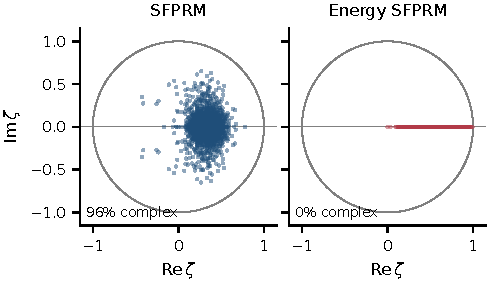
\includegraphics[width=\columnwidth]{figures/spectrum_4x4v2.pdf}\\[2pt]
  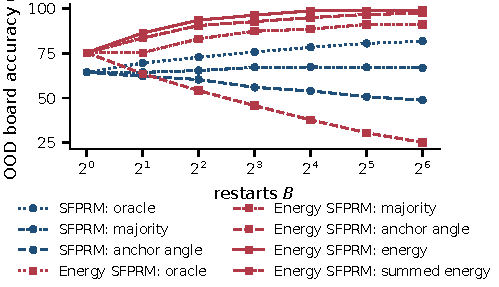
\includegraphics[width=\columnwidth]{figures/restarts_4x4v2.pdf}
  \caption{Codebook variant against SFPRM on $4\times4$ Sudoku. Top: eigenvalues of the tangent
  Jacobian at polished halted OOD states (three puzzles pooled); SFPRM at $\eta=1$, the energy model
  for the damped map at $\eta=1/\lambda_{\max}(\operatorname{Hess}E)$, half its window. Bottom: OOD
  board accuracy against the number of restarts $B$ under the selection rules of
  \cref{prop:voting}; lowest-energy selection coincides with the oracle.}
  \label{fig:codebook}
\end{figure}

The memory term has a probabilistic reading that suggests three further changes. With memories of
fixed norm $\norm{\xi_\mu}=r$, $e^{\beta\ip{\xi_\mu}{z}}$ is, up to normalization, a von
Mises--Fisher density on $\Sph^{d-1}$ with mean direction $\xi_\mu/r$ and concentration $\beta r$
\citep{mardia2000}, so $E_M(z_t)=-\tfrac1\beta\log p(z_t)+\mathrm{const}$ for an equal-weight
vMF mixture centred on the memories, and the memory step is Riemannian gradient ascent on a learned
mixture density. Each term of \eqref{eq:energy} then has a role in a continuous relaxation of a
discrete constraint problem: the injection is the evidence, the attention energy holds the pairwise
constraints, and the memory is a unary potential whose minima are the codebook points. At large
$\beta$ the memory energy of a token approaches $-\max_\mu\ip{\xi_\mu}{z_t}$, a pinning potential
toward the nearest prototype, the learned analogue of the sub-harmonic injection locking that
oscillator Ising machines use to force continuous phases onto discrete values \citep{wang2019oim}.
This motivates the following \emph{codebook variant} of \cref{def:esfprm}.
\emph{Answer codebook and tied readout.} An extra memory term
$E_{\mathrm{ans}}(z)=-\tfrac{\kappa_{\mathrm{ans}}}{\beta_{\mathrm{ans}}}\sum_t\log\sum_{k=1}^{n}e^{\beta_{\mathrm{ans}}\ip{\xi^{\mathrm{ans}}_k}{z_t}}$
on the visible tokens has one unit-norm prototype per output symbol; the readout is
$\mathrm{logits}_t=s\,\Xi^{\mathrm{ans}}z_t$, so the prediction is the prototype the token sits in,
the cross-entropy trains the prototypes directly, and the digit embedding of the input shares the
same prototypes. \emph{Commitment.} $c_t=\max_k\operatorname{softmax}(\beta_{\mathrm{ans}}\Xi^{\mathrm{ans}}z_t)_k$
is a label-free certificate; a token is committed when $c_t>1-\epsilon$, and ``residual below
$\tau$ and every token committed'' is a stronger halting test than the residual alone.
\emph{Annealing.} $\beta$ controls the landscape \citep{ramsauer2021hopfield}: small $\beta$ gives a
single smooth minimum near the mean of the memories, large $\beta$ one minimum per memory. A
schedule $\beta_i=\beta\,\rho^{-(1-\min(i/K,1))}$ over iterations lets coupling and injection act
first and commits tokens late; like an annealed frequency (\cref{sec:oscillatory}) it cannot be
folded into the weight-tied block, and \cref{thm:lyapunov} applies once the schedule has ended.
\emph{Ranking loss.} To make the premise of \cref{prop:voting} hold, training adds, over $R$
restarts of the same puzzle, the hinge $\max(0,E(w^\star_{\mathrm{correct}})-E(w^\star_{\mathrm{wrong}})+m)$
whenever both kinds of halted state occur, so that the energy learns to rank solutions.
\Cref{tab:results} repeats the pilot protocol for the codebook variant and \cref{fig:codebook}
shows its $4\times4$ spectrum and restart curves; \cref{app:pilot} has the training and halting
curves. Five findings.
\emph{The codebook changes the picture.} Without the ranking loss the variant solves $98.0\%$ of
ID and $74.4\%$ of OOD boards on $4\times4$ with one restart, against $97.8\%$ and $65.6\%$ for SFPRM
and $82.4\%$ and $17.2\%$ for the first energy model, and it trains in fewer steps than the first
energy model.
\emph{Energy selection now works.} Selecting the lowest-energy halted state among $B$ restarts
matches the oracle at every $B$: OOD accuracy rises from $75.4\%$ at $B=1$ to $99.0\%$ at $B=64$,
whereas majority voting reaches $91.2\%$ and anchor-angle selection falls to $25.2\%$. SFPRM's best
rule at $B=64$ reaches $67.0\%$ and its oracle $81.8\%$ (\cref{fig:codebook}). The premise of
\cref{prop:voting} holds for the learned energy: whenever a restart finds the solution, it is the
lowest minimum.
\emph{The schedule is necessary, the ranking loss is not.} With $\beta$ fixed at its final value from
the first iteration the variant never leaves the plateau (no board solved, no puzzle halted, in
$2{,}000$ steps): tokens commit to prototypes before attention can propagate the constraints. The ranking loss does not improve
selection, which already matches the oracle without it, and it costs single-restart accuracy
($94.6\%$ / $62.8\%$ with it, although it places the correct state lower in energy for $88\%$ of
training pairs); energy selection behaves well because the readout and the energy share the
prototypes, not because ranking is trained explicitly.
\emph{Commitment certifies.} At the halted state, $75.6\%$ of committed OOD boards are correct and
none of the uncommitted ones. Requiring commitment in the halting test does not help, however: it
lowers board accuracy by $0.4$--$3.0$ points, since almost every state that passes the residual test
is already committed.
\emph{Spectrum and halting.} All eigenvalues at halted states are real, as \cref{prop:real-spectrum}
requires, and Armijo backtracking halts $98\%$ of the OOD puzzles, against $24\%$ for the patience
rule. The learned Hessian remains stiff ($\lambda_{\max}\approx13$), so halting takes a median of
$43$ OOD iterations against $19$ for SFPRM; the $\beta$ schedule does not remove the stiffness.
Replacing only SFPRM's MLP by a tied memory, without any energy, costs a third of the parameters and
some accuracy ($95.8\%$ / $55.0\%$ on $4\times4$, $99.2\%$ / $69.8\%$ on $6\times6$) and leaves
$94\%$ of the eigenvalues complex: the benefits above come from the energy, not from the memory
layer alone.
\emph{$6\times6$.} The first energy model solved no $6\times6$ board; the codebook variant (trained
with the ranking loss) reaches $61.2\%$ ID and $11.0\%$ OOD with one restart, below SFPRM's
$99.8\%$ and $89.2\%$, and its training accuracy was still rising when the $4{,}000$-step budget
ended. Energy selection again tracks the oracle: over $64$ restarts it reaches $100\%$ ID and
$88.2\%$ OOD (oracle $100\%$ and $89.8\%$), against $59.4\%$ for majority voting and $0.4\%$ for
the anchor angle OOD, and just below SFPRM's best rule at $B{=}64$ ($92.8\%$). The spectrum is again
real, halting is again slow (median $103$ OOD iterations), and $98\%$ of committed ID boards are
correct against $52\%$ of uncommitted ones.



% ===========================================================================
\section{Numerical Verification}
\label{sec:numerics}



We checked every identity in double precision on random instances with unit states and inputs, random
weights, and multi-head attention with QK-normalization for \cref{prop:attention}
(\cref{tab:numerics}; setup in \cref{app:numerics}). The exact identities hold to machine precision.
The error of \cref{thm:trotter} falls by a factor of $100$ for every factor-$10$ decrease of
$\varepsilon$, as predicted for $O(\varepsilon^2)$. The Jacobian of \cref{prop:linearization} matches
central finite differences to $10^{-10}$, the accuracy of the differencing.
The energy statements of \cref{sec:energy} were checked in the same way (\cref{app:energy-numerics}).
The closed-form gradient of \cref{prop:energy-gradient} matches automatic differentiation of
\eqref{eq:energy}, the coupling is exactly symmetric, and at a stationary point the Jacobian of
$F_E$ equals $\Id-\operatorname{Hess}E$ with a symmetric Hessian and a purely real spectrum,
whereas a random SFPRM map at a fixed point has a Jacobian with relative asymmetry $0.20$ and
$84\%$ of its eigenvalues off the real axis. The energy never increased in $4{,}000$ gradient
steps at $\eta\in\{0.5,1,1.9\}/\hat L$, with $\hat L$ the largest Hessian eigenvalue found along
descent trajectories, the descent inequality of \cref{thm:lyapunov}(i) held at every step, and
at $\eta=3/\hat L$, outside the window, $54\%$ of the steps increased the energy; the implicit gradient
\eqref{eq:implicit} matches finite differences, conjugate gradient needs $11$ Hessian-vector
products where the Neumann series of truncated BPTT needs $81$ at condition number $6.5$, and the
equilibrium-propagation estimate \eqref{eq:ep} converges with the predicted $O(\beta^2)$ error.

% ===========================================================================
\section{Discussion and Limitations}
\label{sec:discussion}

The correspondence places SFPRM inside the oscillator family as its zero-frequency, single-oscillator,
operator-split member, and places AKOrN's Euler step inside SFPRM's analysis: the existence result,
the damping window and the halting test transfer to the AKOrN form, while the energy and the locking
picture describe what SFPRM's injection does. Several limitations apply. First, the equivalence is a
statement about update rules; readouts, initialization and training differ (\cref{tab:differences}),
so it makes no claim that the two models learn the same functions. Second, the single-step collapse
holds only for small step sizes, which trained SFPRM models do not use (\cref{rem:scope}). Third, the
oscillatory extension and the locking-margin penalty are proposals: we report no experiments on
trained models, and \cref{prop:absorb} shows that a constant frequency alone cannot add expressivity.
Fourth, the verification uses random instances rather than trained weights. Fifth, the energy-based
SFPRM trades expressivity for guarantees: its attention is a conservative field with tied value
matrices and its MLP a tied-weight memory. The pilot studies of \cref{sec:energy-pilot,sec:energy-memory}
are small and single-seeded, on small Sudoku grids where test grids can coincide with training
grids; they show that the codebook variant can match SFPRM and that its energy can rank solutions,
but not that this holds at scale. The learned energies are stiff, so halting remains slower than in
SFPRM, and the $\beta$ schedule voids the descent guarantee during its first iterations. Testing the non-absorbable oscillatory variants and the energy model on
reasoning benchmarks at scale, with conjugate-gradient implicit training and energy voting, is the
natural next step.

% ===========================================================================
\section{Conclusion}
\label{sec:conclusion}

We showed that every update in SFPRM is an AKOrN Euler step with zero natural frequency: exactly at
the level of one iteration, exactly for injection and attention inside it, and to first order for the
iteration as a single step. The two forms share their fixed points and linearization, so SFPRM's
damping window applies to the AKOrN form. The correspondence reads SFPRM's guarantees as oscillator
locking, identifies the absence of an energy function as the main structural difference, and yields
an oscillatory extension with an explicit locking condition, in which a constant frequency reduces to
a reparametrization of the block. Closing the structural gap from the other side, an energy-based
SFPRM makes the recurrent map a gradient step on an explicit energy and thereby gains a Lyapunov
function, a halting bound, a real spectrum at halted states, energy-based voting and equilibrium
propagation. With a codebook memory tied to the readout and an annealed concentration, the learned
energy ranks solutions well enough that energy voting matches the oracle in our pilot.

% ===========================================================================
% Acknowledgements are omitted in the blind submission.

\section*{Impact Statement}

This paper presents work whose goal is to advance the field of Machine Learning. There are many
potential societal consequences of our work, none which we feel must be specifically highlighted here.

\bibliography{references}
\bibliographystyle{icml2026}

% ===========================================================================
\newpage
\appendix
\onecolumn
% ===========================================================================
% APPENDIX (included from main.tex after \appendix\onecolumn)
% ===========================================================================

\section{Mathematical Preliminaries}
\label{app:prelim}

This appendix collects the mathematics needed to read both models. Standard references are
\citet{absil2008} for optimization on manifolds, \citet{kuramoto1984,strogatz2000} for coupled
oscillators, and \citet{lohe2009} for Kuramoto models on higher-dimensional spheres.

\subsection{Spheres, Tangent Spaces and Products of Spheres}

Differentiating $\ip{z(t)}{z(t)}=1$ along a curve on $\Sph^{n-1}$ gives $\ip{\dot z}{z}=0$, so the
tangent space at $z$ is the hyperplane $\tang_z\Sph^{n-1}=\{v:\ip{v}{z}=0\}$. The projector
$\Proj_z=\Id-zz^\top$ of \eqref{eq:proj} is symmetric and idempotent, satisfies $\Proj_zz=0$, and leaves
tangent vectors unchanged. The radial part of a vector changes only its length and is invisible after
normalization; only the tangential part moves a point along the sphere. This decomposition underlies
every identity in the paper.

A state of $M$ unit vectors $z=(z_1,\dots,z_M)$, $z_m\in\Sph^{N-1}$, lives on the product manifold
$(\Sph^{N-1})^M$ of dimension $M(N-1)$, whose tangent space is the product of the factors' tangent
spaces; the projector acts block by block. AKOrN uses $M=C/N$ small factors per position; SFPRM uses one
factor per token ($N=d$), so its state space is $\mathcal S=(\Sph^{d-1})^T$. Rescaling by $1/\sqrt M$
embeds $(\Sph^{N-1})^M$ into $\Sph^{MN-1}$ as the subset on which all blocks have equal norm. On a
sphere a state can neither grow nor vanish, so iterating a map on it is bounded by construction and
only directions carry information; FPRM enforces boundedness by coupling residual coefficients
\citep{movahedi2026fprm}, whereas SFPRM obtains it from the geometry \citep{sfprm}.

The geodesic distance is the angle $\theta=\angle(u,v)$. SFPRM's halting test uses the chordal
quantity $1-\ip{u}{v}=1-\cos\theta=\tfrac12\norm{u-v}^2$. Geodesics are great circles; the one leaving
$u$ in unit tangent direction $e$ is $t\mapsto\cos(t)u+\sin(t)e$, which gives $\Exp_u$. Its inverse
$\Log_u$ follows from $\norm{\Proj_uv}^2=1-\cos^2\theta=\sin^2\theta$. $\Slerp$ is undefined at
antipodal pairs, where the shortest arc is not unique.

\subsection{Retractions and Riemannian Gradients}

A retraction is a smooth map $R_z:\tang_z\Sph^{n-1}\to\Sph^{n-1}$ with $R_z(0)=z$ and identity
derivative at $0$, so it agrees with $\Exp_z$ to first order. Normalization, $R_z(v)=\Ret(z+v)$, is
the retraction used by AKOrN and nGPT. For tangent $v$, $\norm{z+v}^2=1+\norm{v}^2$, hence
\begin{equation}
  \Ret(z+v) = \cos\varphi\,z+\sin\varphi\,\tfrac{v}{\norm{v}},\qquad \tan\varphi=\norm{v}:
\end{equation}
normalization moves along the same great circle as $\Exp_z(v)$ but by the angle $\arctan\norm{v}<\pi/2$
instead of $\norm{v}$. Retraction, exponential map and Slerp therefore differ only in how a step
length is converted into an angle, which is why step sizes can be traded between them exactly.

For a smooth $f$ on $\R^n$, the Riemannian gradient of its restriction to the sphere is
$\grad f(z)=\Proj_z\nabla f(z)$, and Riemannian gradient descent is
$z\leftarrow R_z(-\gamma\grad f(z))$. For the linear potential $f(z)=-\ip{c}{z}$,
$\grad f=-\Proj_zc$ (AKOrN's stimulus); for the geodesic potential $f(z)=\tfrac12\angle(z,x)^2$,
$\grad f=-\Log_zx$ (SFPRM's injection, \cref{prop:injection-gradient}).

\subsection{Antisymmetric Matrices and Rotations}

If $\Omega^\top=-\Omega$ then $\ip{\Omega z}{z}=0$, so $\Omega z$ is tangent and the flow
$\dot z=\Omega z$ preserves the norm; its solution $e^{t\Omega}z(0)$ is a rotation. In a suitable
orthonormal basis $\Omega$ is block diagonal with $2\times2$ blocks $\omega_kR$,
$R=\begin{psmallmatrix}0&-1\\1&0\end{psmallmatrix}$, $R^2=-\Id$, plus a zero row and column when $N$
is odd; each block rotates one plane at the natural frequency $\omega_k$. For odd $N$ a rotation fixes
an axis, and by the hairy-ball theorem every tangent field on $\Sph^{N-1}$ vanishes somewhere. For even
$N$, $\Omega$ can have no zero eigenvalue and $\dot z=\Omega z$ moves every point. This is why AKOrN uses
even $N$, and it is the obstruction to fixed-point existence that SFPRM's injection repairs.

\subsection{The Kuramoto Model in Vector Form}
\label{app:kuramoto}

In $\dot\theta_i=\omega_i+\sum_jK_{ij}\sin(\theta_j-\theta_i)$ \citep{kuramoto1984,strogatz2000},
positive couplings synchronize phases and negative couplings repel them; the order parameter
$re^{i\psi}=\tfrac1n\sum_je^{i\theta_j}$ measures synchrony. A phase-locked state rotates at a common
frequency with constant phase differences and is a fixed point in the co-rotating frame. With
$x_i=(\cos\theta_i,\sin\theta_i)$ we have $\dot x_i=\dot\theta_iRx_i$, where
$Rx_i=(-\sin\theta_i,\cos\theta_i)$ is the unit tangent at $x_i$, and
$\ip{x_j}{Rx_i}=\sin(\theta_j-\theta_i)$. Hence $\Proj_{x_i}x_j=\sin(\theta_j-\theta_i)Rx_i$, which
gives \eqref{eq:kuramoto-vector}. Replacing $\omega_iR$ by an antisymmetric $\Omega_i$, scalar
couplings by matrices $J_{ij}$, and adding an external field $c_i$ that pins oscillators as an injected
signal locks a physical oscillator \citep{adler1946locking} yields \eqref{eq:akorn-ode}
\citep{lohe2009,miyato2025akorn}. The AKOrN implementation rotates with the opposite sign, which only
flips the sign convention of $\omega$.

\subsection{Gradient Flows and Lyapunov Functions}

If $c+Jx=-\nabla E(x)$ and $\Omega=0$, then \eqref{eq:akorn-ode} is the Riemannian gradient flow
$\dot x=-\grad E(x)$, along which
\begin{equation}
  \tfrac{d}{dt}E(x(t))=\ip{\nabla E}{\dot x}=-\norm{\grad E(x)}^2\le0,
\end{equation}
because $\dot x$ is tangent. $E$ is a Lyapunov function, and on a compact state space the flow
settles into the set of stationary points (LaSalle's invariance principle). For
$E(x)=-\tfrac12x^\top Jx-c^\top x$, the condition $c+Jx=-\nabla E$ holds exactly when $J$ is symmetric,
which is the origin of \eqref{eq:akorn-energy}. A rotation $\Omega x$ is not a gradient, and neither is
a non-symmetric coupling such as softmax attention; in those cases no energy is guaranteed.

\subsection{Fixed-Point Iterations and Damping}

A looped model iterates $z_{i+1}=F(z_i)$ and reads its answer at a fixed point $z^\star=F(z^\star)$. If
$F$ is a contraction with constant $q<1$, Banach's theorem gives a unique fixed point and
$\norm{z_i-z^\star}\le q^i\norm{z_0-z^\star}$; this is the form of FPRM's global result
\citep{movahedi2026fprm}. Near a fixed point the error evolves as $e_{i+1}\approx Je_i$ with
$J=\mathrm dF(z^\star)$. The damped (Krasnosel'skii--Mann) iteration
$z_{i+1}=(1-\eta)z_i+\eta F(z_i)$ \citep{mann1953} has the same fixed points for every $\eta\in(0,1]$ and
linearizes to $(1-\eta)\Id+\eta J$, mapping each eigenvalue $\zeta$ to $1+\eta(\zeta-1)$. Since
$|1+\eta(\zeta-1)|^2=1-2\eta(1-\operatorname{Re}\zeta)+\eta^2|\zeta-1|^2$, the mode decays exactly when
$\operatorname{Re}\zeta<1$ and $\eta<2(1-\operatorname{Re}\zeta)/|\zeta-1|^2$. Damping tames rotating
or overshooting modes but no step size helps a mode with $\operatorname{Re}\zeta\ge1$. On the sphere,
$\Slerp_\eta(z_i,F(z_i))$ replaces linear interpolation with the same fixed points and linearization
\citep{sfprm}.

By the implicit function theorem, the parameter gradient at $z^\star$ involves $(\Id-J)^{-1}$. FPRM
and SFPRM avoid forming it: they backpropagate through windows of $K$ iterations, detach the state, and
apply a loss after every window (deep supervision with truncated backpropagation through time). Under
contraction this corresponds to truncating the Neumann series $\sum_{k<K}J^k$ for $(\Id-J)^{-1}$
\citep{movahedi2026fprm}.

\subsection{Transformers on the Sphere}

nGPT \citep{loshchilov2025ngpt} folds a sub-layer output $G(h)$ into the state by
$h\leftarrow\Norm(h+\alpha\odot(\Norm(G(h))-h))$ with per-coordinate eigen learning rates $\alpha$; for
scalar $\alpha$ this is normalized linear interpolation toward $\Norm(G(h))$. Softmax attention,
\begin{equation}
  \Attn(h)_t=\sum_sa_{ts}(h)\,W_OW_Vh_s,\qquad
  a_{ts}(h)=\operatorname{softmax}_s\big(s_{qk}\ip{\Norm(W_Qh_t)}{\Norm(W_Kh_s)}\big),
\end{equation}
is a linear map of the token vectors with state-dependent weights, i.e.\ a coupling
$J_{ts}(h)=a_{ts}(h)W_OW_V$ of the kind AKOrN uses as attention connectivity.

\subsection{Operator Splitting}

For smooth vector fields $A,B$ with flows $\phi^A_\varepsilon,\phi^B_\varepsilon$,
$\phi^B_\varepsilon\circ\phi^A_\varepsilon=\phi^{A+B}_\varepsilon+O(\varepsilon^2)$, with leading
error proportional to the Lie bracket $[A,B]$ \citep{trotter1959}. The same holds for single
retraction steps $z\mapsto R_z(\varepsilon A(z))$, which agree with their flows to first order. A model
that applies stimulus, coupling and nonlinearity as separate small steps is therefore, to first order,
a single step with the summed drive (\cref{thm:trotter}).

% ===========================================================================
\section{Proofs and Additional Statements}
\label{app:proofs}

\paragraph{Attention sub-layer with per-coordinate eigen learning rates.}
The following restates \cref{prop:attention} and adds the per-coordinate case.

\begin{proposition}[Attention sub-layer, full statement]
\label{prop:attention-full}
Let $A_t:=\Attn(h)_t\neq0$, $\hat A_t:=A_t/\norm{A_t}$ and $J_{ts}(h)$ as in \eqref{eq:attn-as-coupling}.
\begin{enumerate}
  \item[(a)] If $\alpha_A=a\mathbf1$ and $1+a(\ip{\hat A_t}{h_t}-1)>0$ (automatic for $a<1/2$), then
  \eqref{eq:ngpt-attn} equals
  $h_t\leftarrow\Ret\big(h_t+\gamma^A_t\Proj_{h_t}\sum_sJ_{ts}(h)h_s\big)$ with
  $\gamma^A_t=a/\big(\norm{A_t}(1+a(\ip{\hat A_t}{h_t}-1))\big)$.
  \item[(b)] If $\alpha_A\in\R^d$, $w_t:=\alpha_A\odot(\hat A_t-h_t)$ and $1+\ip{w_t}{h_t}>0$, then
  \eqref{eq:ngpt-attn} equals
  \begin{equation}
    h_t\leftarrow\Ret\Big(h_t+\tfrac{1}{1+\ip{w_t}{h_t}}\,\Proj_{h_t}\Big[\tfrac{1}{\norm{A_t}}\diag(\alpha_A)\sum_sJ_{ts}(h)h_s-\diag(\alpha_A)h_t\Big]\Big):
  \end{equation}
  the coupling is diagonally preconditioned and a self-drive $-\diag(\alpha_A)h_t$ appears, whose
  tangent part is $-\grad\tfrac12h^\top\diag(\alpha_A)h$ and vanishes when $\alpha_A$ is constant.
\end{enumerate}
\end{proposition}
\begin{proof}
Apply \cref{lem:renorm} with $z=h_t$ and $w=w_t$. For (a),
$\Proj_{h_t}w_t=a\Proj_{h_t}\hat A_t=\tfrac{a}{\norm{A_t}}\Proj_{h_t}\sum_sJ_{ts}h_s$ because
$\Proj_{h_t}h_t=0$, and $1+\ip{w_t}{h_t}=1+a(\ip{\hat A_t}{h_t}-1)$. For (b), $\Proj_{h_t}$ no longer
annihilates $\diag(\alpha_A)h_t$, which produces the self-drive.
\end{proof}

\begin{proposition}[nGPT MLP sub-layer]
\label{prop:mlp}
With $M_t:=\MLP(h)_t\neq0$ and $\hat M_t:=M_t/\norm{M_t}$, \eqref{eq:ngpt-mlp} is the step of
\cref{prop:attention-full} with $\sum_sJ_{ts}h_s$ replaced by the token-wise nonlinear drive $M_t$.
\end{proposition}
\begin{proof}
Identical to \cref{prop:attention-full} with $A_t$ replaced by $M_t$.
\end{proof}

\paragraph{Proof of \cref{thm:trotter} (sketch).}
For a smooth tangent field $v$, $\Ret(y+\varepsilon v(y))=y+\varepsilon v(y)+O(\varepsilon^2)$. By
\cref{lem:slerp},
$\Slerp_{\varepsilon\kappa_0}(z,x)=\Exp_z(\varepsilon\kappa_0\Log_zx)=z+\varepsilon\kappa_0\tfrac{\theta^x}{\sin\theta^x}\Proj_zx+O(\varepsilon^2)$.
Each nGPT sub-layer gives $h\mapsto h+\varepsilon\kappa\Proj_h\hat A+O(\varepsilon^2)$ (or $\hat M$).
Since every intermediate state equals $z+O(\varepsilon)$, evaluating all drives at $z$ costs
$O(\varepsilon^2)$ (Lie--Trotter). Hence $\tilde z=z+\varepsilon\Proj_zV(z)+O(\varepsilon^2)$ and
$\theta_i=O(\varepsilon)$. Then \cref{lem:slerp} gives $\gamma_\eta(\theta_i)=\eta+O(\varepsilon^2)$ and
$z_{i+1}=\Ret(z+\eta\Proj_z\tilde z)+O(\varepsilon^2)=\Ret(z+\eta\varepsilon\Proj_zV(z))+O(\varepsilon^2)$.
\hfill$\square$

\paragraph{Proof of \cref{prop:linearization}.}
Write $v(z):=\Omega z+\Proj_zD(z)$, so $v(z^\star)=0$. Terms involving the derivative of $\gamma$
multiply $v(z^\star)$ and vanish. For a tangent perturbation $u$,
$\mathrm d(\Proj_zD)[u]=\Proj_zJ_Du-\ip{D}{u}z-\ip{D}{z}u$. The middle term is normal and is removed by
the derivative of $\Ret$ at $z^\star$, which equals $\Proj$ because $z^\star+\gamma v(z^\star)=z^\star$
has unit norm. Collecting terms gives the claim. \hfill$\square$

\paragraph{Proof of \cref{cor:window}.}
At a fixed point of SFPRM, $F_\theta(z^\star;x)=z^\star$, so $\mu_t=\ip{z^\star_t}{z^\star_t}=1$ and
$\Proj J_F\Proj-\Id$ restricted to the tangent space equals $J-\Id$. With $\Omega=0$ and
$\gamma\to\eta$, \cref{prop:linearization} gives $\Id+\eta(J-\Id)=(1-\eta)\Id+\eta J$, the
linearization of the $\Slerp$ step reported by \citet{sfprm}. \hfill$\square$

\paragraph{Proof of \cref{prop:adler}.}
Fixed points satisfy $\Omega x+h-\mu x=0$ with $\mu:=\ip{h}{x}$. In plane $k$, $\Omega_k=\omega_kR'$
with $R'=\begin{psmallmatrix}0&1\\-1&0\end{psmallmatrix}$, $R'^2=-\Id$, and
$(\omega_kR'-\mu\Id)^{-1}=-(\omega_kR'+\mu\Id)/(\omega_k^2+\mu^2)$. Hence
$x_k=(\omega_kR'+\mu\Id)h_k/(\omega_k^2+\mu^2)$, and since $R'h_k\perp h_k$ and $\norm{R'h_k}=\norm{h_k}$,
\begin{equation}
  \norm{x}^2=g(\mu):=\sum_k\frac{\norm{h_k}^2}{\omega_k^2+\mu^2}.
\end{equation}
Consistency holds automatically: $\ip{h}{x}=\sum_k\mu\norm{h_k}^2/(\omega_k^2+\mu^2)=\mu\,g(\mu)$, which
equals $\mu$ whenever $g(\mu)=1$. Fixed points therefore correspond to solutions of $g(\mu)=1$. The
function $g$ is even, strictly decreasing in $|\mu|$, tends to $0$ as $|\mu|\to\infty$, and satisfies
$g(0)=\sum_k\norm{h_k}^2/\omega_k^2$, so a solution exists if and only if $g(0)\ge1$. \hfill$\square$

% ===========================================================================
\section{Numerical Verification Setup}
\label{app:numerics}

All checks used NumPy in double precision. % TODO: release the verification scripts as supplementary material.
\begin{itemize}
  \item \textbf{\Cref{lem:renorm,lem:slerp}.} $5{,}000$ random draws in $d=64$: unit $z$ and $v$, damping
  $\eta\sim\mathcal U(0.02,1)$, and nGPT-style updates $w=\alpha\odot(A-z)$ with unit $A$ and
  $\alpha_i\sim\mathcal U(0,0.5)$; only draws satisfying the positivity conditions enter the maxima.
  \item \textbf{\Cref{prop:attention}.} $T=6$ tokens, $d=16$, $H=2$ heads with QK-normalization
  (logit scale $4$), scalar eigen learning rate $a=0.3$. The identity
  $\Attn(h)_t=\sum_sJ_{ts}(h)h_s$ holds to $2.2\times10^{-16}$.
  \item \textbf{\Cref{thm:trotter}.} The same tokens with one nGPT-style layer (attention and an MLP
  $h\mapsto\tanh(W_1h)$), $\eta=1$, all $\kappa=1$; the error between the split iteration and the single
  step is reported at $\varepsilon\in\{10^{-1},10^{-2},10^{-3}\}$.
  \item \textbf{\Cref{prop:linearization}.} One token in $d=6$ with
  $F(z)=\Ret(\tanh(Wz+b)+1.2z)$, $\gamma=0.5$, and either $\Omega=0$ or three rotation planes with
  frequencies $(0.3,0.2,0.1)$. Fixed points were found by iterating $50{,}000$ steps (residual
  $<10^{-16}$); Jacobians were compared with central differences of step $10^{-6}$ on the tangent space.
  \item \textbf{\Cref{prop:adler}.} $N=4$ with plane frequencies $(1.0,0.6)$, random drives rescaled so
  that $\sum_k\norm{h_k}^2/\omega_k^2\in\{0.6,0.9,0.99,1.01,1.1,2\}$, step $\gamma=0.05$, $40{,}000$ steps
  from three random initializations. For values $\ge1.01$ the final tangent speed was below
  $10^{-15}$; for values $\le0.99$ it stayed above $7\times10^{-2}$.
\end{itemize}

% ===========================================================================
\section{Proofs for the Energy-Based SFPRM}
\label{app:energy-proofs}

\paragraph{Proof of \cref{prop:energy-gradient}.}
Write $q^k_t=W_Q^ku_t$, $k^k_s=W_K^kz_s$ and $\ell^k_{ts}=\beta_k\ip{q^k_t}{k^k_s}$. For the Euclidean
gradient of $E_A$ with respect to $u_t$ only the terms of head $k$ in which $t$ is the query index
contribute, and $\partial_{u_t}\big[-\tfrac{\sigma_k}{\beta_k}\log\sum_{s\neq t}e^{\ell^k_{ts}}\big]
=-\sigma_k\sum_{s\neq t}a^k_{ts}(W_Q^k)^\top k^k_s=-\sigma_k\sum_{s\neq t}a^k_{ts}M_kz_s$. For $z_s$
only terms in which $s$ is the key index contribute, one for every query $t\neq s$, giving
$-\sigma_k\sum_{t\neq s}a^k_{ts}(W_K^k)^\top q^k_t=-\sigma_k\sum_{t\neq s}a^k_{ts}M_k^\top u_t$;
renaming indices yields the key-path sum in \eqref{eq:grad-z}. The bilinear term gives
$-\kappa_CC^\top u_t$ and $-\kappa_CCz_t$, the memory term gives
$-\kappa_M\sum_\mu\operatorname{softmax}_\mu(\beta_M\Xi u_t)\,\xi_\mu$, and the injection term gives
$-\kappa_0\Log_{z_t}x_t$ after projection (\cref{prop:injection-gradient}). The Riemannian gradient
on a product of spheres is the token-wise projection $\Proj_{w_t}$ of the Euclidean gradient
(\cref{app:prelim}), which proves \eqref{eq:grad-z}--\eqref{eq:grad-u}. In the flat variant
$u_t=z_t$ and the two attention contributions to token $t$ add to
$\sum_{s\neq t}\big(a^k_{ts}M_k+a^k_{st}M_k^\top\big)z_s$, so $J_{ts}=\sum_k\sigma_k(a^k_{ts}M_k+a^k_{st}M_k^\top)$
and $J_{st}^\top=\sum_k\sigma_k(a^k_{st}M_k^\top+a^k_{ts}M_k)=J_{ts}$. \hfill$\square$

\paragraph{Proof of \cref{thm:lyapunov}.}
\emph{Existence of $L$.} $E_A$, $E_C$ and $E_M$ are real-analytic on $\R^{2Td}$, so their
restrictions to the compact manifold $(\Sph^{d-1})^{2T}$ have bounded Riemannian Hessians, and for the
exponential retraction $t\mapsto E(\Exp_w(tv))$ has second derivative
$\operatorname{Hess}E(\gamma(t))[\dot\gamma,\dot\gamma]\le\lambda_{\max}(\operatorname{Hess}E)\norm v^2$,
which gives the inequality with $L=\sup\lambda_{\max}(\operatorname{Hess}E)$ by Taylor's theorem
\citep[Ch.~10]{boumal2023}. For the injection term, on $\Sph^{d-1}$ the Hessian of
$\tfrac12\angle(\cdot,x)^2$ at angle $\theta\in(0,\pi)$ has eigenvalue $1$ along the geodesic to $x$
and $\theta\cot\theta\le1$ on its orthogonal complement; at the antipode the function has a concave
corner, so its second derivative along any geodesic is bounded above by $1$ in the distributional
sense and the inequality holds with the contribution $\kappa_0$ at every $w$ with no token antipodal
to its input, which is the exceptional set of the theorem; for the chordal injection
$\sum_t(1-\ip{z_t}{x_t})$, AKOrN's stimulus potential, the Hessian is bounded by $1$ everywhere and
no exception is needed.
\emph{(i)} Take $v=-\eta\grad E(w_i)$:
$E(w_{i+1})\le E(w_i)-\eta\norm{\grad E(w_i)}^2+\tfrac L2\eta^2\norm{\grad E(w_i)}^2=E(w_i)-c_\eta\norm{\grad E(w_i)}^2$.
\emph{(ii)} Summing (i) over $i<N$ and using that $E$ is continuous on a compact set, hence bounded
below by $\min E$, gives $c_\eta\sum_{i<N}\norm{\grad E(w_i)}^2\le E(w_0)-\min E$ for every $N$. Hence
$\grad E(w_i)\to0$, and by continuity of $\grad E$ every accumulation point is stationary. If the
halting test has not fired before iteration $N$ then $\norm{\grad E(w_i)}\ge\max_t\norm{\grad_{w_t}E(w_i)}\ge\tau_g$
for all $i<N$, so $Nc_\eta\tau_g^2\le E(w_0)-\min E$. \emph{(iii)} By (i) and $v=-\eta\grad E$, the
iteration is a descent method with exact gradient direction and sufficient decrease, so the
Łojasiewicz argument of \citet{absil2005analytic}, applied in a chart around an accumulation point
where $E$ is real-analytic, shows that the sequence has finite length and converges. For decaying
step sizes $\eta_i\in[\eta_{\min},\eta]$, (i) holds with $c_{\eta_i}\ge\min(c_{\eta_{\min}},c_\eta)$
because $c$ is concave in $\eta$ on $(0,2/L)$. \hfill$\square$

\paragraph{Proof of \cref{prop:real-spectrum}.}
$F_E$ is the generalized AKOrN step of \cref{def:gen-akorn} with $\Omega=0$, $\gamma=1$, drive
$D=-\nabla E$ and the exponential retraction in place of normalization; at a fixed point the two
retractions have the same derivative because both equal the identity on the tangent space to first
order and the step vanishes. \Cref{prop:linearization} with $J_D=-\nabla^2E$ and
$\mu_t=\ip{D_t}{w^\star_t}=-\ip{\nabla_{w_t}E}{w^\star_t}$ gives
$\mathrm dF_E=\Id-\big(\Proj\nabla^2E\,\Proj-\operatorname{M}_{\mu'}\big)$ with
$\mu'_t=\ip{\nabla_{w_t}E}{w^\star_t}$, and the bracket is the Riemannian Hessian of $E$ on the
product of spheres \citep[Sec.~5.4]{absil2008}. It is self-adjoint on the tangent space because
$\Proj\nabla^2E\,\Proj$ is symmetric and $\operatorname{M}_{\mu'}$ is a token-wise multiple of the
identity. By \cref{cor:window} the $\Slerp$ step linearizes to $(1-\eta)\Id+\eta\,\mathrm dF_E=\Id-\eta\operatorname{Hess}E$.
The spectral theorem gives real eigenvalues $h$ of the Hessian and $\zeta=1-h$ of $\mathrm dF_E$. The
mode decays iff $|1-\eta h|<1$ iff $0<h<2/\eta$; all modes decay iff $\operatorname{Hess}E\succ0$ and
$\eta<2/\lambda_{\max}$, and for real $\zeta$ the window $2(1-\operatorname{Re}\zeta)/|\zeta-1|^2$
of \cref{cor:window} equals $2/h$. If some $h<0$ then $|1-\eta h|>1$ for every $\eta>0$. \hfill$\square$

\paragraph{Eigen learning rates as a preconditioner.}
Let $D=\diag(\alpha)\succ0$ be fixed and replace the step by $w\leftarrow\Exp_w(-\eta\,\Proj D\,\grad E(w))$.
Then $\ip{\grad E}{\Proj D\grad E}=\ip{\grad E}{D\grad E}\ge\alpha_{\min}\norm{\grad E}^2$, so the
direction is a descent direction and \cref{thm:lyapunov} holds with $c_\eta$ replaced by
$\eta(\alpha_{\min}-\eta L\alpha_{\max}^2/2)$. At a stationary point the Jacobian is
$\Id-\eta(\Proj D\Proj)\operatorname{Hess}E$, and $(\Proj D\Proj)\operatorname{Hess}E$ restricted to
the tangent space is similar to $S^{1/2}\operatorname{Hess}E\,S^{1/2}$ with $S=\Proj D\Proj\succ0$ on
the tangent space, which is symmetric, so the spectrum stays real.

\paragraph{Proof of \cref{prop:voting}.}
The residual bound is \cref{def:esfprm}. Energy selection with $\sigma_k=\kappa_C=\kappa_M=0$ is
anchor-angle selection. Let $w^\sharp$ be the global minimizer with basin $\mathcal B$ of measure
$p>0$. A restart in $\mathcal B$ halts at a $\tau_g$-stationary point $w^{(b)}$ in the basin, with
$E(w^{(b)})\le\min E+\delta(\tau_g)$, where the halting slack $\delta$ vanishes with $\tau_g$. Any other
halted state is within the same slack of a stationary value, which by assumption exceeds $\min E+2\delta$
(the gap condition of the proposition),
so $w^{(b)}$ has the smallest energy among the halted states and decodes correctly. The probability
that none of $B$ starts falls in $\mathcal B$ is $(1-p)^B\to0$. \hfill$\square$

\paragraph{Implicit gradient and equilibrium propagation.}
At an attracting halted state, $\grad E(w^\star;\theta)=0$ with $\operatorname{Hess}E(w^\star)\succ0$,
so by the implicit function theorem (in a chart) $w^\star(\theta)$ is smooth and differentiating the
stationarity condition gives $\operatorname{Hess}E\,\frac{\mathrm dw^\star}{\mathrm d\theta}+\frac{\partial\grad E}{\partial\theta}=0$.
Hence $\frac{\mathrm d\ell}{\mathrm d\theta}=\ip{\grad\ell}{\frac{\mathrm dw^\star}{\mathrm d\theta}}=-\ip{\operatorname{Hess}E^{-1}\grad\ell}{\partial_\theta\grad E}$,
which is \eqref{eq:implicit}. With $J=\mathrm dF_E=\Id-\operatorname{Hess}E$ the matrix
$(\Id-J)^{-1}$ of \cref{app:prelim} is $\operatorname{Hess}E^{-1}$, and the truncated Neumann series
of truncated BPTT becomes $\eta\sum_{k<K}(\Id-\eta\operatorname{Hess}E)^k$, whose error after $K$
terms is $(1-\eta\lambda_{\min})^K$, i.e.\ $K=O(\kappa\log(1/\epsilon))$ for $\eta=1/\lambda_{\max}$,
against $O(\sqrt\kappa\log(1/\epsilon))$ for conjugate gradient \citep[Thm.~5.5]{nocedal2006}. For
\eqref{eq:ep}, let $G(\theta,\beta):=\min_wE(w;\theta)+\beta\ell(w)=E(w^\star_\beta;\theta)+\beta\ell(w^\star_\beta)$.
By the envelope theorem $\partial_\theta G=\partial_\theta E(w^\star_\beta;\theta)$ and
$\partial_\beta G=\ell(w^\star_\beta)$; equality of mixed partial derivatives gives
$\frac{\mathrm d}{\mathrm d\theta}\ell(w^\star_\beta)=\frac{\mathrm d}{\mathrm d\beta}\partial_\theta E(w^\star_\beta;\theta)$,
and $\beta=0$ yields \eqref{eq:ep} \citep{scellier2017ep}; the argument uses only stationarity on the
manifold.

% ===========================================================================
\section{Pilot Experiment: Energy-Based versus Standard SFPRM}
\label{app:pilot}

\paragraph{Tasks.}
Sudoku of size $4\times4$ ($2\times2$ boxes, $T=16$) and $6\times6$ ($2\times3$ boxes, $T=36$).
Puzzles are generated by filling a random grid with a randomized backtracking solver and removing
cells in random order while the puzzle keeps a unique solution, until a target number of clues is
reached. For $6\times6$, training uses $12{,}000$ puzzles with $14$--$22$ clues (mean $18.0$); the
in-distribution (ID) test set has puzzles from the same range and the out-of-distribution (OOD) test
set puzzles with $8$--$13$ clues (mean $11.1$), mirroring the easy/hard split used for AKOrN. For
$4\times4$, training uses $400$ puzzles with $7$--$10$ clues and the OOD test set has $4$--$6$
clues; since only $288$ distinct $4\times4$ grids exist, test grids can coincide with training grids,
and the $4\times4$ task measures constraint propagation rather than generalization across grids.
Evaluation uses $500$ puzzles per test set. Each cell is a token; the input embedding is
$x_t=\Norm(e_{\mathrm{digit}(t)}+Wp_t)$ with a learned digit table (blank included) and a learned
linear map $W$ of the row/column/box one-hot features $p_t$, shared by both models. The readout is
linear, $s\,W_{\mathrm{out}}z_t+b$, and the loss is the cross-entropy over all cells.

\paragraph{Models.}
\emph{SFPRM}: $d=64$, $D=2$ nGPT layers with $H=4$ heads, QK-normalized attention with a learned
logit scale per head, a GELU MLP of width $4d$, per-coordinate eigen learning rates initialized at
$0.25$, injection $\lambda=0.5$, $\Slerp$ damping; PSF parameters. \emph{Energy SFPRM}
(\cref{def:esfprm}, hidden variant): $d=64$, $H=8$ heads of dimension $8$ with signed weights
initialized at $\pm0.2$ (alternating), $W_Q,W_K$ with entries of standard deviation $1/\sqrt d$,
logit scales $\beta_k=d/\sqrt{d_h}$, $K=1024$ memories with $\beta_M=\sqrt d$, $\kappa_0=0.5$,
$\kappa_C=0.5$, $\kappa_M=0.1$, geodesic injection; PEN parameters. All positive scales are
softplus-parametrized and learned.

\paragraph{Training.}
Both models are trained identically: AdamW (learning rate $2\times10^{-3}$, weight decay $0.01$ on
matrices, cosine decay, $200$ warm-up steps, gradient clipping at $1$), batch $128$,
$4{,}000$ steps on $6\times6$ ($400$ for SFPRM and $2{,}000$ for the energy model on $4\times4$,
each run until its training accuracy had saturated), random unit-norm initial states, deep supervision with two windows of $K=8$ iterations at $\eta=1$
and the state detached between windows, exactly the recipe described for FPRM and SFPRM. For the
energy model each training iteration uses Armijo backtracking on $E$ (acceptance constant
$10^{-4}$, at most four halvings, step size treated as a constant), which keeps the training
dynamics inside the descent regime of \cref{thm:lyapunov}; without it, energy increases in up to
half of the iterations once the attention sharpens, and the model does not learn.

\paragraph{Evaluation.}
At test time both models run the damped loop from random unit-norm states for at most $128$
iterations with the chordal halting test at $\tau_c=10^{-4}$, $\eta$ starting at $1$ and halved
after $3$ iterations without residual improvement (patience rule, minimum $1/64$); for the energy
model we report Armijo backtracking in place of the patience rule, and use it for the spectrum and
restart measurements as well; the patience rule, which starts at $\eta=1$, far outside the energy
model's window, halts only about half of the puzzles within $128$ iterations. \emph{Iterations to halt}
are counted over puzzles that halt. \emph{Spectrum}: for $20$ ID and $20$ OOD puzzles the halted
state is polished in double precision (continuing the damped iteration until the residual is below
$10^{-12}$ or for $2{,}000$ steps), and the Jacobian of the proposal map $F$ on the tangent space
is computed by automatic differentiation in an orthonormal tangent basis; we report the fraction of
eigenvalues with $|\operatorname{Im}\zeta|>10^{-8}$, $\max|\operatorname{Im}\zeta|$, the relative
asymmetry $\norm{J-J^\top}_{\max}/\norm{J}_{\max}$, and the damping window of \cref{cor:window}.
\emph{Restarts}: for $B\in\{1,2,4,\dots,64\}$ independent random starts per puzzle we select one
halted state by (a) the final energy $E(w^\star;x)$, (b) the energy summed over the first $32$
iterations, as AKOrN does, (c) the anchor-angle potential $\Phi_x(z^\star)$, which is available in
plain SFPRM, (d) majority vote over decoded boards, and report board accuracy; the oracle is the
fraction of puzzles for which any of the $B$ restarts is correct.

\paragraph{Results of the first energy model.}
\Cref{tab:pilot} and \cref{fig:pilot} summarize the comparison of \cref{sec:energy-pilot}. Four
observations. \emph{Accuracy and training cost.} The energy model learns both tasks, but needs several times more
optimization steps than SFPRM to leave the ``clues only'' plateau (\cref{fig:training}), and at an
equal budget it is behind: on $4\times4$ it reaches 82.4\% ID and 17.2\% OOD against 97.8\% and
65.6\% for SFPRM, and on $6\times6$ it does not leave the plateau within the $4{,}000$-step budget in which SFPRM reaches $99.8\%$ ID and $89.2\%$ OOD (cell accuracy $72\%$, no board solved). Without the three design choices of
\cref{sec:energy-design} and Armijo backtracking in training it does not leave the plateau at all.
\emph{Spectrum.} At every polished halted state the energy model's Jacobian is symmetric to
machine precision and all eigenvalues are real, whereas 96.4\% of SFPRM's eigenvalues are complex
with imaginary parts up to 0.61 (\cref{fig:pilot}, left). The learned energy is stiff, however:
$\lambda_{\max}(\operatorname{Hess}E)\approx 12.2$, so the admissible step is
$\eta<2/\lambda_{\max}\approx 0.16$ rather than SFPRM's $\approx 1.40$, and the slow modes of a
stiff Hessian make halting \emph{slower}, not faster: 68 / 114 iterations (median / p90, OOD) against
19 / 45 for SFPRM. Real eigenvalues remove the rotational obstruction of \cref{cor:window}, but the
condition number of the learned Hessian decides the halting time, and nothing in the training
objective controls it. \emph{Halting rule.} With Armijo backtracking the energy model halts
81.8\% of the OOD puzzles within $128$ iterations and the energy never increases; the patience rule,
which starts at $\eta=1$, halts about half as many (\cref{tab:pilot-full}).
\emph{Energy selection.} Energy voting does not help here: selecting the lowest-energy halted
state among $B=64$ restarts gives 12.4\% OOD on $4\times4$, below the single-restart accuracy, while
majority voting gives 20.6\% and the oracle 36.0\%. The premise of \cref{prop:voting} fails, as the
lowest minima of the learned energy are not the correct boards; deep supervision never asks them
to be. Anchor-angle selection fails in the same way for both models.

\begin{table}[h]
  \caption{Pilot comparison on $4\times4$ and $6\times6$ Sudoku ($500$ test puzzles each; board
  accuracy in \%; one restart unless stated; iterations to halt at $\tau_c=10^{-4}$ over halted
  puzzles, median / 90th percentile; spectrum of $\mathrm dF$ at polished halted OOD states). The
  energy model uses Armijo backtracking at test time, SFPRM the patience rule.}
  \label{tab:pilot}
  \vskip 0.1in
  \begin{center}
  \begin{footnotesize}
  \setlength{\tabcolsep}{2.5pt}
  \begin{tabular}{@{}lcccc@{}}
    \toprule
     & \multicolumn{2}{c}{$4\times4$} & \multicolumn{2}{c}{$6\times6$} \\
    \cmidrule(lr){2-3}\cmidrule(lr){4-5}
     & SFPRM & Energy & SFPRM & Energy \\
    \midrule
    Parameters ($\times10^3$) & 101 & 79 & 101 & 80 \\
    Steps to $90\%$ train acc.\ & 200 & 1250 & 400 & $>4000$ \\
    Board acc.\ ID & 97.8 & 82.4 & 99.8 & 0.0 \\
    Board acc.\ OOD & 65.6 & 17.2 & 89.2 & 0.0 \\
    Halted, OOD ($\le128$ it.) & 73.4 & 81.8 & 90.6 & 30.4 \\
    Iterations to halt, OOD & 19 / 45 & 68 / 114 & 19 / 37 & 102 / 122 \\
    Complex $\zeta$ & 96.4 & 0.0 & 96.4 & 0.0 \\
    $\max|\operatorname{Im}\zeta|$ & 0.61 & $0$ & 0.65 & 0.02 \\
    $\lambda_{\max}(\operatorname{Hess}E)$ & -- & 12.2 & -- & 17.9 \\
    Window (\cref{cor:window}) & 1.40 & 0.16 & 1.33 & 0.12 \\
    OOD, $B{=}64$: energy & -- & 12.4 & -- & 0.0 \\
    OOD, $B{=}64$: anchor & 48.8 & 20.4 & 92.8 & 0.0 \\
    OOD, $B{=}64$: majority & 67.0 & 20.6 & 90.6 & 0.0 \\
    OOD, $B{=}64$: oracle & 81.8 & 36.0 & 93.8 & 0.0 \\
    \bottomrule
  \end{tabular}
  \end{footnotesize}
  \end{center}
  \vskip -0.1in
\end{table}

\begin{figure}[h]
  \centering
  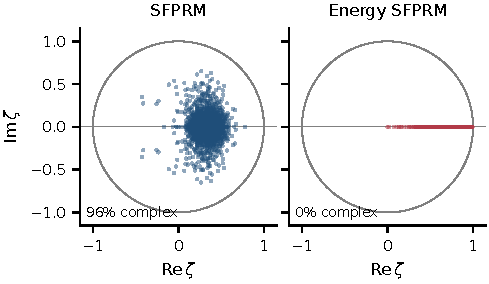
\includegraphics[width=0.48\textwidth]{figures/spectrum_4x4.pdf}\hfill
  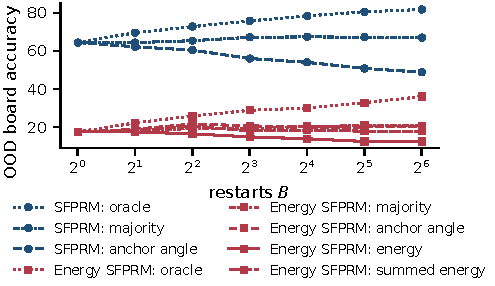
\includegraphics[width=0.48\textwidth]{figures/restarts_4x4.pdf}
  \caption{First energy model against SFPRM on $4\times4$ Sudoku. Left: eigenvalues of the tangent Jacobian at polished halted OOD states
  (three puzzles pooled); SFPRM at $\eta=1$, the energy model for the damped map at
  $\eta=1/\lambda_{\max}(\operatorname{Hess}E)$, half its window. Right: OOD board accuracy against
  the number of restarts $B$ under the selection rules of \cref{prop:voting}.}
  \label{fig:pilot}
\end{figure}

\paragraph{Full results.}
\Cref{tab:pilot-full} lists the ID and OOD numbers for both tasks and both halting rules, and
\cref{fig:training} shows the training curves and the distribution of iterations to halt.
On $4\times4$ the energy model solves $82.4\%$ of ID and $17.2\%$ of OOD boards after $2{,}000$
steps (SFPRM: $97.8\%$ and $65.6\%$ after $400$), halting $93.6\%$ and $81.8\%$ of the puzzles within
$128$ iterations under Armijo backtracking against $47\%$ and $28\%$ under the patience rule. On
$6\times6$ its training cell accuracy rises from $58\%$ to $73\%$ over $4{,}000$ steps but no board
is solved, so the restart curves of \cref{fig:pilot6} are flat at zero; the spectrum and halting
measurements at its halted states remain valid and show the same picture as on $4\times4$: real
eigenvalues (the ID Jacobians have relative asymmetry $\le4\times10^{-2}$ and no complex pair; on OOD
the polishing step did not reach the $10^{-12}$ residual within $2{,}000$ iterations at the small
admissible step for all puzzles, leaving imaginary parts up to $0.09$ in one of six cases), a stiff
Hessian with $\lambda_{\max}\approx14$--$18$, a window of $0.12$--$0.16$, and halting after $88$
(ID) and $102$ (OOD) iterations at the median, against $11$ and $19$ for SFPRM. The $4\times4$
restart curves show the selection rules in detail: energy selection decreases monotonically with
$B$ ($84.8\%$ at $B=1$ to $78.8\%$ at $B=64$ ID; $17.4\%$ to $12.4\%$ OOD), the summed energy and
the anchor angle are flat, majority voting gains little, and the oracle rises to $95.2\%$ ID and
$36.0\%$ OOD, so the restarts do contain correct boards that no available score identifies.

\begin{table}[h]
  \caption{Full pilot results (board accuracy in \%, $500$ puzzles per set; iterations to halt
  over halted puzzles). Pat.: patience rule; Arm.: Armijo backtracking on $E$.}
  \label{tab:pilot-full}
  \vskip 0.1in
  \begin{center}
  \begin{small}
  \begin{tabular}{@{}llcccccc@{}}
    \toprule
    Task & Model (rule) & Acc.\ ID & Acc.\ OOD & Halted ID & Halted OOD & It.\ ID (med/p90) & It.\ OOD (med/p90) \\
    \midrule
    $4\times4$ & SFPRM (Pat.) & 97.8 & 65.6 & 98.2 & 73.4 & 13 / 18 & 19 / 45 \\
    $4\times4$ & Energy (Pat.) & 80.2 & 21.4 & 47.0 & 28.0 & 49 / 67 & 50 / 67 \\
    $4\times4$ & Energy (Arm.) & 82.4 & 17.2 & 93.6 & 81.8 & 61 / 100 & 68 / 114 \\
    $6\times6$ & SFPRM (Pat.) & 99.8 & 89.2 & 99.8 & 90.6 & 11 / 13 & 19 / 37 \\
    $6\times6$ & Energy (Pat.) & 0.0 & 0.0 & 2.4 & 1.0 & 54 / 97 & 67 / 118 \\
    $6\times6$ & Energy (Arm.) & 0.0 & 0.0 & 62.0 & 30.4 & 88 / 117 & 102 / 122 \\
    \bottomrule
  \end{tabular}
  \end{small}
  \end{center}
\end{table}

\begin{figure}[h]
  \centering
  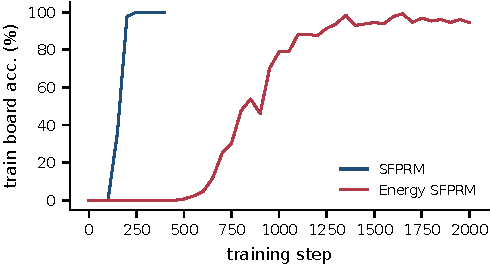
\includegraphics[width=0.48\textwidth]{figures/training_4x4.pdf}\hfill
  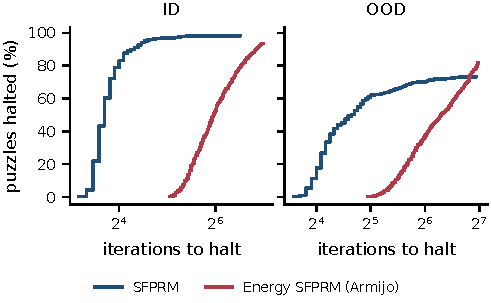
\includegraphics[width=0.48\textwidth]{figures/halting_4x4.pdf}\\[4pt]
  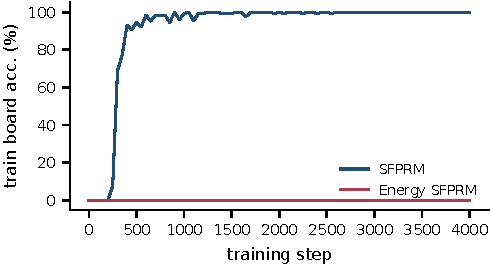
\includegraphics[width=0.48\textwidth]{figures/training_6x6.pdf}\hfill
  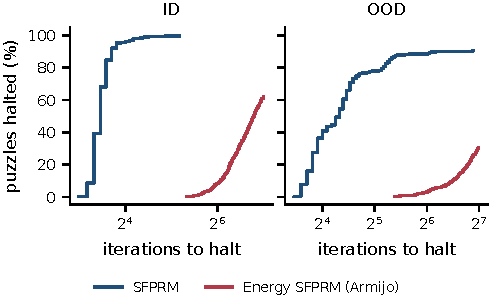
\includegraphics[width=0.48\textwidth]{figures/halting_6x6.pdf}
  \caption{Training curves (left; train board accuracy, logged every $50$ steps) and cumulative
  distribution of iterations to halt (right; SFPRM with the patience rule, the energy model with
  Armijo backtracking) on $4\times4$ (top) and $6\times6$ (bottom) Sudoku.}
  \label{fig:training}
\end{figure}

\begin{figure}[h]
  \centering
  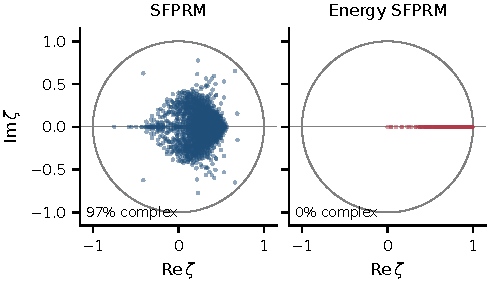
\includegraphics[width=0.48\textwidth]{figures/spectrum_6x6.pdf}\hfill
  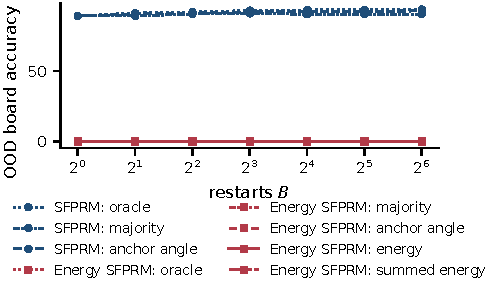
\includegraphics[width=0.48\textwidth]{figures/restarts_6x6.pdf}
  \caption{$6\times6$ pilot: Jacobian spectra at polished halted OOD states (left) and OOD board
  accuracy against the number of restarts (right), as in \cref{fig:pilot}, for the first energy model.}
  \label{fig:pilot6}
\end{figure}

\paragraph{Codebook variant.}
The codebook runs of \cref{tab:results} use the hidden-token energy model of \cref{app:pilot} with the answer
codebook on the visible tokens ($\kappa_{\mathrm{ans}}=0.5$, $\beta_{\mathrm{ans}}=\sqrt d$ at the
end of the schedule, prototypes initialized as orthonormal directions and kept at unit norm), the
tied readout with a learned scale, the digit embedding tied to the prototypes, the $\beta$ schedule
$\rho=8$ over the first $K=8$ iterations applied to both memory terms (so the energy is only
non-increasing after iteration $8$, and the energy-increase counter of \cref{app:pilot} is not
meaningful during the schedule), the ranking loss with weight $0.1$, margin $1$ and $R=2$ restarts
per puzzle (batch $64\times2$) when enabled, and otherwise the training recipe of
\cref{app:pilot}; $2{,}000$ steps on $4\times4$ and $4{,}000$ on $6\times6$. On $6\times6$ only the
variant with the ranking loss was trained, at learning rate $10^{-3}$; a first run at
$2\times10^{-3}$ diverged after $500$ steps (loss rising from $0.93$ to $1.34$) and was stopped. A
further $4\times4$ ablation fixes $\beta$ at its final value from the first iteration (with the
ranking loss): it stays on the clue-only plateau for all $2{,}000$ steps, with $65\%$ ID and $49\%$
OOD cell accuracy, no board solved and no puzzle halted within $128$ iterations. The memory-MLP ablation of SFPRM uses $256$ tied
memories with a learned $\beta$ in place of the GELU MLP in both nGPT layers. Evaluation adds a third
halting rule, Armijo backtracking with the commitment requirement, and reports the commitment
statistics at the Armijo-halted state. With the commitment requirement, board accuracy is
$97.6\%$ ID and $71.4\%$ OOD for the codebook model ($98.0\%$ and $74.4\%$ without it) and $93.6\%$
and $61.6\%$ with the ranking loss ($94.6\%$ and $62.8\%$). \Cref{fig:v2} shows the training curves and halting distributions of the
codebook variant against SFPRM, and its $6\times6$ spectrum and restart curves.

\begin{figure}[h]
  \centering
  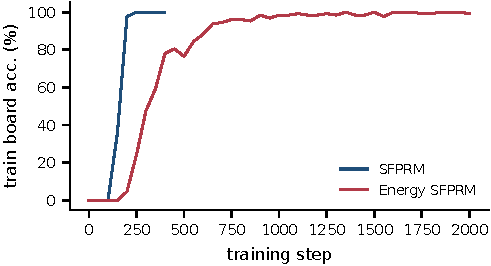
\includegraphics[width=0.48\textwidth]{figures/training_4x4v2.pdf}\hfill
  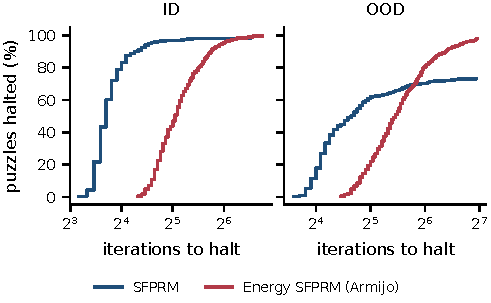
\includegraphics[width=0.48\textwidth]{figures/halting_4x4v2.pdf}\\[4pt]
  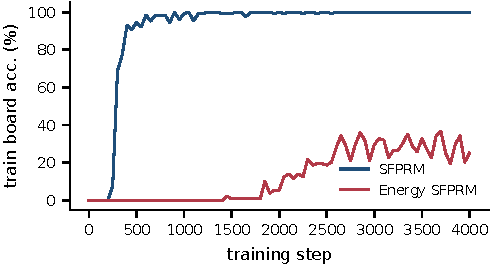
\includegraphics[width=0.48\textwidth]{figures/training_6x6v2.pdf}\hfill
  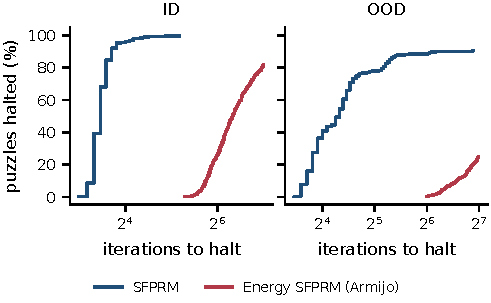
\includegraphics[width=0.48\textwidth]{figures/halting_6x6v2.pdf}\\[4pt]
  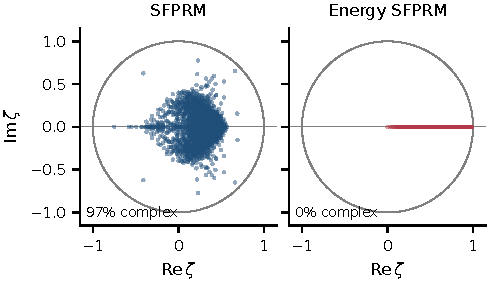
\includegraphics[width=0.48\textwidth]{figures/spectrum_6x6v2.pdf}\hfill
  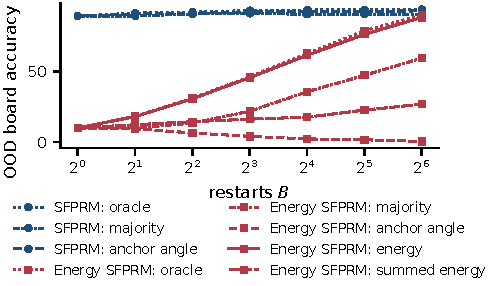
\includegraphics[width=0.48\textwidth]{figures/restarts_6x6v2.pdf}
  \caption{Codebook variant (``Energy SFPRM'') against SFPRM. Top: $4\times4$ training curves and
  iterations to halt (``Codebook'' column of \cref{tab:results}). Middle and bottom: $6\times6$
  training curves, iterations to halt, spectra at halted OOD states and OOD accuracy against
  restarts (``$+$rank'' column).}
  \label{fig:v2}
\end{figure}

% ===========================================================================
\section{Numerical Verification of the Energy Statements}
\label{app:energy-numerics}

All checks use the model of \cref{def:esfprm} with random weights in double precision: $T=6$ tokens,
$d=16$, $H=2$ heads of dimension $8$, $K=24$ memories, $\kappa_0=1$, signed head weights
$\sigma=(0.3,-0.3)$, $\beta_k=2$, $\kappa_M=0.5$, $\beta_M=3$, and the geodesic injection; inputs
$x$ are normalized embeddings of random clues. Scripts are included with the submission.
\begin{itemize}
  \item \textbf{\Cref{prop:energy-gradient}.} The closed-form drive \eqref{eq:grad-z}--\eqref{eq:grad-u}
  is compared with $-\Proj_w\nabla E$ from automatic differentiation on $200$ random states for the
  flat model and $100$ for the hidden model. The coupling matrices $J_{ts}$ of the flat model are
  assembled explicitly and compared with $J_{st}^\top$, and $\Proj_z\sum_sJ_{ts}z_s$ with the attention
  part of the drive.
  \item \textbf{\Cref{prop:real-spectrum}.} A stationary point is found by iterating
  \eqref{eq:esfprm-step} with $\eta=0.2$ until $\norm{\grad E}<10^{-14}$ ($765$ iterations). The
  tangent Jacobian of $F_E$ (automatic differentiation in an orthonormal basis of the tangent space)
  is compared with $\Id-\operatorname{Hess}E$, where the Riemannian Hessian is
  $\Proj\nabla^2E\,\Proj-\operatorname{M}_\mu$, and with central finite differences of step $10^{-6}$
  along tangent directions. The Hessian eigenvalues lie in $[0.21,1.90]$. For comparison, a random
  one-layer SFPRM map (scalar eigen learning rates $0.3$, $\lambda=0.5$) is iterated to a fixed point
  (residual $<10^{-30}$) and its tangent Jacobian is analysed in the same way.
  \item \textbf{\Cref{thm:lyapunov}.} $\hat L$ is the largest Riemannian Hessian eigenvalue over $50$
  random states ($2.23$) and over the states and midpoints visited by $20$ descent trajectories of
  $20$ steps ($3.05$). $200$ trajectories of $20$ steps are then run at
  $\eta\in\{0.5,1,1.9,3\}/\hat L$; at the three step sizes inside the window the energy never
  increased and the inequality of (i) held at every step (worst slack $-5.9\times10^{-8}$ at
  $1.9/\hat L$), while at $3/\hat L$ the energy increased in $54\%$ of the steps.
  \item \textbf{\Cref{eq:implicit}.} At a stationary point with Hessian condition number $6.5$ and a
  linear loss $\ell(w)=\ip{\omega}{w}$ with random $\omega$, the adjoint system is solved exactly, by
  conjugate gradient, and by the truncated Neumann series $\eta\sum_{k<K}(\Id-\eta\operatorname{Hess}E)^k$
  with $\eta=1/\lambda_{\max}$; the iteration counts to relative error $10^{-3}$ are $7$ and $40$ and
  to $10^{-6}$ they are $11$ and $81$. The resulting derivative of $\ell(w^\star)$ with respect to
  $\kappa_0$ is compared with central finite differences of step $10^{-5}$ through the re-solved
  stationary point.
  \item \textbf{\Cref{eq:ep}.} The nudged minimizer of $E+\beta\ell$ is found by the same iteration
  and \eqref{eq:ep} is evaluated one-sided and centered for $\beta\in\{10^{-1},10^{-2},10^{-3}\}$;
  the relative errors are $2.5$, $0.34$, $0.034$ (one-sided, $O(\beta)$) and $0.050$, $0.0010$,
  $1.1\times10^{-5}$ (centered, $O(\beta^2)$).
\end{itemize}


\end{document}
